\documentclass{article}
\usepackage{amsthm,amsmath,amsfonts,natbib,mathtools,custom_math}
\usepackage[hscale=0.7,vscale=0.8]{geometry}

\usepackage{subfigure}
\usepackage{graphicx}
\usepackage{hyperref}
\usepackage{authblk}

\usepackage{yhmath}

\bibliographystyle{plainnat}

\title{Faithful Variable Screening for High-Dimensional Convex Regression}

%\author{
%Min Xu, Minhua Chen, John Lafferty
%}

\author[1]{Min Xu}
\author[2,3]{Minhua Chen}
\author[2,3]{John Lafferty}

\affil[1]{Machine Learning Department, Carnegie Mellon University}
\affil[2]{Department of Statistics, University of Chicago}
\affil[3]{Department of Computer Science, University of Chicago}


% ENVIRONMENTS
% \numberwithin{equation}{section}
% \theoremstyle{plain}
% \newtheorem{theorem}{Theorem}[section]
% \newtheorem{corollary}{Corollary}[section]
% \newtheorem{proposition}{Proposition}[section]
% \newtheorem{lemma}{Lemma}[section]
% \newtheoremstyle{remark}{\topsep}{\topsep}%
%      {\normalfont}% Body font
%      {}           % Indent amount (empty = no indent, \parindent = para indent)
%      {\bfseries}  % Thm head font
%      {.}          % Punctuation after thm head
%      {.5em}       % Space after thm head (\newline = linebreak)
%      {\thmname{#1}\thmnumber{ #2}\thmnote{ #3}}% Thm head spec
% \theoremstyle{remark}
% \newtheorem{remark}{Remark}[section]
% \newtheorem{example}{Example}[section]
% \newtheorem{assumption}{Assumption}[section]
% \newtheorem{definition}{Definition}[section]

\newcommand{\fix}{\marginpar{FIX}}
\newcommand{\new}{\marginpar{NEW}}
\DeclareMathOperator{\rank}{rank}
\DeclareMathOperator{\diag}{diag}
\DeclareMathOperator{\trace}{trace}
\DeclareMathOperator{\pr}{Prob}
\DeclareMathOperator{\cov}{Cov}
\newcommand{\EE}[1]{\mathbb{E}({#1})}
\def\interleave{|\kern-.25ex|\kern-.25ex|}
\def\interleavesub{|\kern-.15ex|\kern-.15ex|}
\newcommand{\nnorm}[1]{\interleave {#1} \interleave}
\newcommand{\nnormsub}[1]{\interleavesub {#1} \interleavesub}
\newcommand{\nNorm}[1]{\left|\kern-.25ex\left|\kern-.25ex\left| {#1}\right|\kern-.25ex\right|\kern-.25ex\right|}
\newcommand{\norm}[1]{\left\|{#1}\right\|}
%\newcommand{\trnorm}[1]{\norm{{#1}}_{\mathrm{tr}}}
\newcommand{\trnorm}[1]{\norm{{#1}}_{*}}
\newcommand{\spnorm}[1]{\norm{{#1}}_{\mathrm{sp}}}
\newcommand{\frnorm}[1]{\norm{{#1}}_{\mathrm{F}}}
%\newcommand{\trnnorm}[1]{\nnorm{{#1}}_{\mathrm{tr}}}
\newcommand{\trnnorm}[1]{\nnorm{{#1}}_{*}}
\newcommand{\spnnorm}[1]{\nnorm{{#1}}_{\mathrm{sp}}}
\newcommand{\spnnormsub}[1]{\nnormsub{{#1}}_{\mathrm{sp}}}
\newcommand{\frnnorm}[1]{\nnorm{{#1}}_{\mathrm{F}}}
\newcommand{\Norm}[1]{\left\|{#1}\right\|}
%\newcommand{\Trnorm}[1]{\Norm{{#1}}_{\mathrm{tr}}}
\newcommand{\Trnorm}[1]{\Norm{{#1}}_{*}}
\newcommand{\Spnorm}[1]{\Norm{{#1}}_{\mathrm{sp}}}
\newcommand{\Frnorm}[1]{\Norm{{#1}}_{\mathrm{F}}}
%\newcommand{\Trnnorm}[1]{\nNorm{{#1}}_{\mathrm{tr}}}
\newcommand{\Trnnorm}[1]{\nNorm{{#1}}_{*}}
\newcommand{\Spnnorm}[1]{\nNorm{{#1}}_{\mathrm{sp}}}
\newcommand{\Frnnorm}[1]{\nNorm{{#1}}_{\mathrm{F}}}
\newcommand{\colspan}[1]{\mathrm{colspan}\left({#1}\right)}
\def\myllangle{\langle\mspace{-4mu}\langle\mspace{1mu}}
\def\myrrangle{\mspace{1mu}\rangle\mspace{-4mu}\rangle}

\numberwithin{equation}{section}
\theoremstyle{plain}
\newtheorem{theorem}{Theorem}[section]
\newtheorem{stheorem}{Theorem}
\newtheorem{corollary}{Corollary}[section]
\newtheorem{proposition}{Proposition}[section]
\newtheorem{lemma}{Lemma}[section]
\newtheoremstyle{remark}{\topsep}{\topsep}%
     {\normalfont}% Body font
     {}           % Indent amount (empty = no indent, \parindent = para indent)
     {\bfseries}  % Thm head font
     {.}          % Punctuation after thm head
     {.5em}       % Space after thm head (\newline = linebreak)
     {\thmname{#1}\thmnumber{ #2}\thmnote{ #3}}% Thm head spec
\theoremstyle{remark}
\newtheorem{remark}{Remark}[section]
\newtheorem{example}{Example}[section]
\newtheorem{assumption}{Assumption}[section]
\newtheorem{definition}{Definition}[section]

% min's macros
\mathchardef\mh="2D

% John's macros
\def\X{\mathcal{X}}
\def\comma{\unskip,~}
\def\truep{p^*}
\def\div{\|\,}
\long\def\comment#1{}
\def\reals{{\mathbb R}}
\def\R{\reals}
\def\P{{\mathbb P}}
\def\E{{\mathbb E}}
\def\Cov{\mathop{\text{Cov}}}
\def\supp{\mathop{\text{supp}\kern.2ex}}
\def\argmin{\mathop{\text{\rm arg\,min}}}
\def\arginf{\mathop{\text{\rm arg\,inf}}}
\def\argmax{\mathop{\text{\rm arg\,max}}}
\let\tilde\widetilde
\def\csd{${}^*$}
\def\mld{${}^\dag$}
\def\dos{${}^\ddag$}
\def\W{\widetilde Y}
\def\Z{\widetilde X}
\let\hat\widehat
\let\tilde\widetilde
\def\given{{\,|\,}}
\def\ds{\displaystyle}
\def\bs{\backslash}
\def\1{{(1)}}
\def\2{{(2)}}
\def\pn{{(n)}}
\def\ip{{(i)}}
\def\Xbar{\overline{X}}
\def\except{\backslash}
\def\npn{\mathop{\textit{NPN\,}}}
\def\i{{(i)}}
\def\cE{{\mathcal{C}}}
\def\cM{{\mathcal{M}}}
\def\cF{{\mathcal{F}}}
\def\cP{{\mathcal{P}}}
\def\cG{{\mathcal{G}}}
\def\tr{\mathop{\text{tr}}}
\long\def\comment#1{}
\def\ti#1{#1}
\def\titi#1{\textit{#1}}
\def\cram{{\sc cram}}
\def\spam{{\small\sc SpAM}}
\def\diag{\mathop{\rm diag}}
\def\ones{\mathbf{1}}
\def\threebars{\mbox{$|\kern-.25ex|\kern-.25ex|$}}
\def\fatnorm#1{\threebars #1 \threebars}
\def\rank{\mathop{\rm rank}}
\def\S{\mathcal{S}}
\def\H{\mathcal{H}}
\def\K{{K}}
\def\rank{\mathop{\rm rank}}
\def\half{{1/2}}
\def\Y{\mathbb{Y}}
\def\M{\mathbb{M}}
\def\F{\mathbb{F}}
\def\pinv{{-1}}
%\def\ones{\mathds{1}}
%\def\ones{1}
\def\Res{Z}
\def\Proj{P}
\def\cN{{\mathcal N}}
\def\cT{{\mathcal H}}
\def\coloneqq{:=}
\def\mathbf#1{\mbox{\boldmath $#1$}} 
\def\bar#1{\overline{#1}}






\begin{document}

% min's macros
\mathchardef\mh="2D

% John's macros
% \def\X{\mathcal{X}}
% \def\comma{\unskip,~}
% \def\truep{p^*}
% \def\div{\|\,}
% \long\def\comment#1{}
% \def\reals{{\mathbb R}}
% \def\P{{\mathbb P}}
% \def\E{{\mathbb E}}
% \def\Cov{\mathop{\text{Cov}}}
% \def\supp{\mathop{\text{supp}\kern.2ex}}
% \def\argmin{\mathop{\text{\rm arg\,min}}}
% \def\arginf{\mathop{\text{\rm arg\,inf}}}
% \def\argmax{\mathop{\text{\rm arg\,max}}}
% \let\tilde\widetilde
% \def\csd{${}^*$}
% \def\mld{${}^\dag$}
% \def\dos{${}^\ddag$}
% \def\W{\widetilde Y}
% \def\Z{\widetilde X}
% \let\hat\widehat
% \let\tilde\widetilde
% \def\given{{\,|\,}}
% \def\ds{\displaystyle}
% \def\bs{\backslash}
% \def\1{{(1)}}
% \def\2{{(2)}}
% \def\pn{{(n)}}
% \def\ip{{(i)}}
% \def\Xbar{\overline{X}}
% \def\except{\backslash}
% \def\npn{\mathop{\textit{NPN\,}}}
% \def\i{{(i)}}
% \def\cE{{\mathcal{C}}}
% \def\cM{{\mathcal{M}}}
% \def\cF{{\mathcal{F}}}
% \def\cP{{\mathcal{P}}}
% \def\cG{{\mathcal{G}}}
% \def\tr{\mathop{\text{tr}}}
% \long\def\comment#1{}
% \def\ti#1{#1}
% \def\titi#1{\textit{#1}}
% \def\cram{{\sc cram}}
% \def\spam{{\small\sc SpAM}}
% \def\diag{\mathop{\rm diag}}
% \def\ones{\mathbf{1}}
% \def\threebars{\mbox{$|\kern-.25ex|\kern-.25ex|$}}
% \def\fatnorm#1{\threebars #1 \threebars}
% \def\rank{\mathop{\rm rank}}
% \def\S{\mathcal{S}}
% \def\H{\mathcal{H}}
% \def\K{{K}}
% \def\rank{\mathop{\rm rank}}
% \def\half{{1/2}}
% \def\Y{\mathbb{Y}}
% \def\M{\mathbb{M}}
% \def\F{\mathbb{F}}
% \def\pinv{{-1}}
% %\def\ones{\mathds{1}}
% %\def\ones{1}
% \def\Res{Z}
% \def\Proj{P}
% \def\cN{{\mathcal N}}
% \def\cT{{\mathcal H}}
% \def\coloneqq{:=}
% \def\mathbf#1{\mbox{\boldmath $#1$}} 
% \def\bar#1{\overline{#1}}




\maketitle

\begin{abstract}
We consider the problem of estimating a convex function of several variables from noisy values of the function at a finite sample of input points. Convex function estimation is subject to the curse of dimensionality where the sample size necessary for consistent estimation increases exponentially with the dimensionality of the observed variables $p$. However, if the function is sparse, with $s << p$ relevant variables, then one could achieve consistency in the high-dimensional setting by first identifying the $s$ variables. We develop a faithful screening procedure to compute a set $S$ that contains the $s$ relevant variables. Our approach is a two-stage method that estimates a sum of $p$ one-dimensional convex functions, followed by one-dimensional concave regression fits on the residuals. The method is based on quadratic programming, and in contrast to standard sparse additive models, requires no tuning parameters for smoothness. Under appropriate assumptions, we prove that the procedure is faithful in the population setting, yielding no false negatives, and we give a finite sample statistical analysis. In addition, we introduce algorithms for efficiently carrying out the required quadratic programs. The approach leads to significant computational and statistical advantages over fitting a full model, and provides an effective, practical approach to variable screening in convex regression.

\end{abstract}
\vskip10pt

% \tableofcontents

\section{Introduction}


Shape restrictions such as monotonicity, convexity, and concavity
provide a natural way of limiting the complexity of many statistical
estimation problem.  Shape-constrained estimation is not as well
understood as more traditional nonparametric estimation involving
smoothness constraints.  For instance, as of this writing, the minimax
rate of convergence for multivariate convex regression has yet to be
rigorously established in full generality.  Even the one-dimensional
case is challenging, and has been of recent interest
\citep{guntusen:13}.

In this paper we study the problem of variable selection in convex
regression.  Assuming that the regression function is convex and
sparse, our goal is to identify the relevant variables.  We show that
it suffices to estimate a sum of $p$ one-dimensional convex functions,
leading to significant computational and statistical advantages.  This
is in contrast to general nonparametric regression, where fitting an
additive model can result in false negatives.  Our approach is based
on a two-stage quadratic programming procedure.  In the first stage,
we fit an convex additive model, imposing a sparsity penalty.  In the
second stage, we fit a concave function on the residual for each
variable.  As we demonstrate, this perhaps non-intuity second stage is
in general necessary.  Our first result is that this procedure is
faithful in the population setting, meaning that it results in no
false negatives, under mild assumptions on the density of the
covariates.  Our second result is a finite-sample statistical analysis
of the procedure, where we upper bound the statistical rate of
convergence.  Each stage of the method requires quadratic programming.
An additional contribution is to show how these quadratic programs can
be forumlated to be more scalable.  Simulations demonstrate the method
performs in a manner that is consistent with our analysis.

Variable selection for nonparametric
regression under smoothness constraints is difficult without
making additional strong assumptions. 
\cite{lafferty2008rodeo} show that computationally
efficient, near minimax-optimal estimation is possible, but in ambient
dimensions that scale only as $p = O(\log n)$; see also \cite{BertinLecue}.  This is in contrast
to the $p=O\bigl(e^{n^c}\bigr)$ scaling enjoyed by sparse linear
models \cite{Wain:09a}. \citet{dalalyan:12} achieve exponential scaling $p=O(e^n)$
under certain Fourier smoothness conditions, but require
that the number of relevant variables $s$ must be less than $\log n$.

Approximating the regression function by a sum of one-dimensional
functions, known as sparse additive models \citep{Ravikumar:09}, is a
practical alternative to fully nonparametric function estimation.  
Sparse additive models have been further studied in by \cite{Meier09},
and by \cite{Raskutti:12}.  But 
the additive assumption is limited.  In particular, the natural idea
of first selecting the single variable effects, then the pairwise
effects, and so on, does not in general lead to consistent variable
selection.  In other words, the general nonparametric model is not
additively faithful.  Remarkably, the additional assumption of
convexity does lead to consistent variable selection, as we show
here. In addition, we show that the high dimensional scaling $n =
O\big(\textrm{poly}(s) \log p\big)$ is achievable for sparse convex
additive models. Thus, with respect to variable selection, the
geometric convexity constraint is quite different from the smoothness
constraints imposed in traditional nonparametric regression.

A key to our approach is the observation that least squares
nonparametric estimation under convexity constraints is equivalent to
a finite dimensional quadratic program.  Specifically, the infinite
dimensional optimization 
\begin{align}
\begin{split}
\text{minimize} & \quad \sum_{i=1}^n (Y_i - m(x_i))^2 \\
\text{subject to} &  \quad m:\reals^p\rightarrow\reals\ \text{is
  convex}
\end{split}
\end{align}
is precisely equivalent to the finite dimensional quadratic
program 
\begin{align}
\begin{split}
\label{eq:outer}
\text{minimize}_{h, \beta} & \;\; \sum_{i=1}^n (Y_i - h_i)^2 \\
\text{subject to} & \;\; h_j \geq h_i + \beta_i^T (x_j-x_i),\; \text{for
    all $i,j$}.
\end{split}
\end{align}
%\end{equation}
%See \cite{Boyd04}, Section 6.5.5.
Here $h_i$ is the estimated function value $m(x_i)$, and the vectors
$\beta_i \in \reals^d$ represent supporting hyperplanes to the
epigraph of $m$.  Importantly, this finite dimensional quadratic program does
not have tuning parameters for smoothing the function. Such parameters are the bane
of nonparametric estimation.

Estimation of convex functions arises naturally in several
applications.  Examples include geometric programming \cite{Boyd04},
computed tomography \cite{Prince:90}, target reconstruction
\cite{Lele:92}, image analysis \cite{Golden:06} and circuit design
\cite{Hannah:12}.  Other applications include queuing theory
\cite{Chen:01} and economics, where it is of interest to estimate
concave utility functions \cite{Pratt:68}.  See \cite{Lim:12} for
other applications.  

Beyond cases where the assumption of convexity is
natural, we offer that the convexity assumption is attractive as a
tractable, nonparamametric relaxation of the linear model.  In
addition to the lack of tuning parameters, other than the
regularization parameter $\lambda$ to control the level of sparsity,
the global convexity assumption leads to effective, scalable algorithms.  We
demonstrate use of our approach on experiments with standard
regression data sets, in a comparison with sparse linear models
(lasso).

%In the following section we give a high-level summary of our technical
%results, including additive faithfulness, variable selection 
%consistency, and high dimensional scaling.  In Section~X...

\def\mathbf#1{\mbox{\boldmath $#1$}} 



% DO NOT CHANGE; RefTex variables -minx

%%% Local Variables: ***
%%% mode:latex ***
%%% TeX-master: "paper.tex" ***
%%% End: ***
\input{related_work}
\def\x{\mathbf{x}}

\section{Overview of Results}

In this section we provide a high-level description of our technical
results.  Our presentation is intended to give the reader
an overview of our results and their significance.  The 
full technical details, the precise statement of the results,
and their detailed proofs are provided in following sections.

Our results address three problems.  The first is to develop
a procedure based on an additive approximation for identifying
relevant variables in convex regression.  To this end,
we prove a result that shows when and how the additive approximation
be used without introducing false negatives in the population setting.  The
second result concerns the efficient implementation of
the quadratic programs required by the procedure.  
Finally, the third problem we consider is the finite-sample
behavior of our proposed method.  

We first establish some notation, to be used throughout the remainder 
of the paper.
If $\mathbf{x}$ is a vector, we use $\mathbf{x}_{-k}$ to denote the
vector with the $k$-th coordinate removed. If $\mathbf{v} \in \R^n$, then
$v_{(1)}$ denotes the smallest coordinate of $\mathbf{v}$ in
magnitude, and $v_{(j)}$ denotes the $j$-th smallest; $\mathbf{1}_n \in \R^n$
is the all ones vector. If $X \in \R^p$ and $S \subset
\{1,...,p\}$, then $X_S$ is the subvector of $X$ restricted to
the coordinates in $S$. Given $n$ samples $X^{(1)},...,X^{(n)}$, we use
$\bar{X}$ to denote the empirical average. Given a random variable
$X_k$ and a scalar $x_k$, we use $\E[\cdot \given x_k]$ as a shorthand
for $\E[ \cdot \given X_k = x_k]$.


\subsection{Additive faithfulness}

The starting point for our approach is the observation that least squares
nonparametric estimation under convexity constraints is equivalent to
a finite dimensional quadratic program.  Specifically, the infinite
dimensional optimization 
\begin{align}
\begin{split}
\text{minimize} & \quad \sum_{i=1}^n (Y_i - f(\x_i))^2 \\
\text{subject to} &  \quad f:\reals^p\rightarrow\reals\ \text{is
  convex}
\end{split}
\end{align}
is equivalent to the finite dimensional quadratic
program 
\begin{align}
\begin{split}
\text{minimize}_{f, \beta} & \;\; \sum_{i=1}^n (Y_i - f_i)^2 \\
\text{subject to} & \;\; f_j \geq f_i + \beta_i^T (\x_j-\x_i),\; \text{for
    all $i,j$}.
\end{split}
\end{align}
See \cite{Boyd04}, Section 6.5.5.
Here $f_i$ is the estimated function value $f(\x_i)$, and the vectors
$\beta_i \in \reals^d$ represent supporting hyperplanes to the
epigraph of $f$.  Importantly, this finite dimensional quadratic program does
not have tuning parameters for smoothing the function. 

For general regression, using an additive approximation for variable
selection may make errors.  In particular, the nonlinearities in the
regression function may result in an additive component being wrongly
zeroed out.  Surprisingly, this will not happen for convex regression
under appropriate conditions.

A differential function $f$ depends on variable $x_k$ if
$\partial_{x_k} f \neq 0$ with probability greater than zero.  An additive approximation is given by
\begin{equation}
\{f_k^*\}, \mu^* \coloneqq \argmin_{f_1,\ldots, f_p, \mu} \Bigl\{ 
             \E ( f(X) - \mu - \sum_{k=1}^p f_k(X_k))^2 
         \,:\, \E f_k(X_k) = 0 \Bigr\}.
\end{equation}
We say that $f$ is \textit{additively faithful} in case $f^*_k = 0$
implies that $f$ does not depend on coordinate $k$.
% We can define the support $\trm{supp}(f) \coloneqq \{ k \,:\,
% \trm{$k$ is relevant to $f$}\}$. Let $f^* = \sum_{k=1}^s$, then $f$
% is additively faith if $\trm{supp}(f) = \trm{supp}(f^*)$.
Additive faithfulness is a desireable property,
since it implies that an additive approximation may allow us to 
screen out irrelevant variables.

Our first result shows that convex multivariate functions are
additively faithful
under the following assumption on the distribution of the data.
\begin{definition}
  Let $p(\mathbf{x})$ be a density supported on $[0,1]^p$.  Then $p$
  satisfies the \emph{boundary-points condition} if, for all $j$, and
  for all $\mathbf{x}_{-j}$:
\[
\frac{\partial p(\mathbf{x}_{-j} \given x_j)}{\partial x_j}  =  
\frac{\partial^2 p(\mathbf{x}_{-j} \given x_j)}{\partial x_j^2} = 0
\quad \trm{at $x_j = 0$ and $x_j = 1$}.
\]
\end{definition}

As discussed in Section~\ref{sec:additivefaithful}, this is a relatively weak condition. 
Our first result is that this condition suffices in the population
setting of convex regression.

\begin{theorem}
  Let $p$ be a positive density supported on $C=[0,1]^s$ that
  satisfies the boundary-points property. If $f$ is convex and twice
  differentiable, then $f$ is additively faithful under $p$.
\end{theorem}

% We give the full proof in Section~\ref{sec:faithful_proof} of the
% Appendix, but pause here to provide some intuition. 

Intuitively, an additive approximation zeroes out variable $k$ when, fixing $x_k$, every
``slice'' of $f$ integrates to zero. We prove this result
by showing that ``slices'' of convex
functions that integrate to zero cannot be ``glued together'' while
still maintaining convexity.

While this shows that convex functions are additively faithful, it is difficult to
estimate the optimal additive functions $f^*_k$'s.  The difficulty
is that $f^*_k$ need not be
a convex function, as we show through a counterexample
in Section~\ref{sec:additivefaithful}.   
Since the true regression function $f$ is convex, it is natural to ask
when it is sufficient to estimate an convex additive model.  
Unfortunately, a convex additive approximation is not generally
faithful.  In other words, it could be that $f^*_k\equiv 0$
even for a relevant variable $x_k$.  But our next result
shows that this type of error can be detected by fitting 
a \textit{concave} function to the residual.  If the
concave fit to the residual is zero, we can then safely
mark $x_k$ as an irrelevant variable.

\begin{theorem}
Suppose $p(\mathbf{x})$ is a positive
density on $C=[0,1]^p$ and satisfies the boundary-points
condition. Suppose that $f$ is convex and twice-differentiable.
and that $\partial_{x_k} f$, $\partial_{x_k} p( \mathbf{x}_{-k}
\given x_k )$, and $\partial_{x_k}^2 p( \mathbf{x}_{-k} \given x_k)$
are all continuous as functions on $C$.\\
Define
\begin{equation}
\{ f^*_k \}_{k=1}^p,\mu^* = \arg\min \Big \{
\E\big( f(X) - \mu - \sum_{k=1}^s f_k(X_k) \big)^2 \,:\, f_k \in
\mathcal{C}^1, \, \E f_k(X_k) = 0 \Big \}
\end{equation} where $\mathcal{C}^1$ is the set of univariate convex
functions, and
\begin{equation}
g^*_k = \arg\min \Big\{ \E\big( f(X) -
\sum_{k' \neq k} f^*_{k'}(X_{k'}) - g_k \big)^2 \,:\, g_k \in \mh
\mathcal{C}^1, \E g_k(X_k) = 0 \Big\},
\end{equation}
with $\mh{}\mathcal{C}^1$ denoting the set of univariate concave
function.  Then, $f^*_k = 0$ and $g^*_k = 0$ implies that $f$ does not
depend on $x_k$, i.e., $\partial_{x_k} f(\mathbf{x}) = 0$ with
probability one.
\end{theorem}

This result suggests a two-stage screening
procedure for variable selection. In the first stage we fit a sparse \emph{convex}
additive model.  In the second stage we
fit a concave function $\hat g_k$ to the residual for each variable
having a zero convex component $\hat f_k$.  If both $\hat f_k = 0$ and
$\hat g_k = 0$, we remove variable $x_k$.  
Our next results concern the optimizations involved, and their finite
sample statistical performance.


\subsection{Optimization}

\subsection{Finite-sample analysis}







\section{Additive Faithfulness}
\label{sec:additivefaithful}

For general regression, an additive approximation may result in a
relevant variable being incorrectly marked as irrelevant. Such
mistakes are inherent to the approximation and may persist even in
the population setting.  In this section we give
examples of this phenomenon, and then show how the convexity
assumption
changes the behavior of the additive approximation. We begin
with a lemma that characterizes the components of the additive approximation under mild conditions.

% OLD lemma, requires product distribution
% \begin{lemma}
% \label{lem:general_int_reduction}
% Let $F$ be a product distribution on $\mathbf{C}=[0,1]^s$ with density function $p$ which is positive on $\mathbf{C}$. Let
% $X=(X_1,...,X_p) \sim F$. Let $f: \mathbf{C} \rightarrow \R$ be an
% integrable function.
% Let 
% \begin{equation}
% f_k^*, \mu^* \coloneqq \argmin_{f_1,\ldots, f_p, \mu} \Bigl\{ \E \bigl( f(X)  -
%  \sum_{k=1}^s f_k(X_k) -\mu \bigr)^2 
%         \,:\, \E f_k(X_k) = 0\Bigr\}.
% \end{equation}
% Then $\mu^* = \E f(X)$ and $f^*_k(x_k) = \E[ f(X) \given x_k] - \E f(X)$ and this solution is unique.
% \end{lemma}


\begin{lemma}
\label{lem:general_int_reduction}
Let $F$ be a distribution on $C=[0,1]^p$ with a positive density
function $p$. Let $f: C \rightarrow \R$ be an integrable function,
and define 
\begin{equation}
f^*_1,...,f^*_p, \mu^* \coloneqq 
\arg\min \left\{ \E \Bigl( f(X) - \mu - \sum_{k=1}^p f_k(X_k)\Bigr)^2 \,:\,
\E f_k(X_k) = 0,\; \forall k=1,\ldots, p \right\}.
\end{equation}
Then $\mu^* = \E f(X)$,
\begin{equation}
\label{eq:backfit}
f^*_k(x_k) = \E\Bigl[ f(X) - \sum_{k' \neq k} f^*_{k'}(X_{k'}) \given
x_k\Bigr] - \E f(X) 
\end{equation}
and this solution is unique.
\end{lemma}


Lemma~\ref{lem:general_int_reduction} follows from the stationarity
conditions of the optimal solution.   This result is known, and
criterion \eqref{eq:backfit} is used in the backfitting
algorithm for fitting additive models.   We include 
a proof as our results build on it.
% perhaps include this in an appendix??

\begin{proof}
  Let $f^*_1,...,f^*_p, \mu^*$ be the minimizers as defined.  We first
  show that the optimal $\mu$ is $\mu^* = \E f(X)$ for any $f_1, ...,
  f_k$ such that $\E f_k(X_k) = 0$. This follows from the stationarity
  condition, which states that $\mu^* = \E[ f(X) - \sum_k f_k(X_k)] =
  \E[ f(X) ]$. Uniqueness is apparent because the second derivative is
  strictly larger than zero and strong convexity is guaranteed.

  We now turn our attention toward the $f^*_k$s.  It must be that
  $f^*_k$ minimizes 
\begin{equation}
\E\Bigl[ \big( f(X) - \mu^* - \sum_{k' \neq k}
  f^*_{k'} (X_{k'}) - f_k (X_k) \big)^2\Bigr]
\end{equation}
subject to $\E f_k(X_k) = 0$.
Fixing $x_k$, we will show that the value 
\begin{equation}
\E[ f(X) - \sum_{k' \neq k}
f_{k'}(X_{k'}) \given x_k] - \mu^*
\end{equation} 
uniquely minimizes
\begin{equation}
\min_{ f_k(x_k) } \int_{\mathbf{x}_{-k}} p(\mathbf{x}) 
         \Big( f(\mathbf{x}) - \sum_{k' \neq k} f^*_{k'} (x_{k'}) - f_k (x_k) -\mu^*\Big)^2 
                 d \mathbf{x}_{-k}.
\end{equation}
The first-order optimality condition gives us
\begin{align}
\int_{\mathbf{x}_{-k}} p(\mathbf{x}) f_k(x_k) d \mathbf{x}_{-k} &= 
  \int_{\mathbf{x}_{-k}} p(\mathbf{x}) 
      ( f(\mathbf{x})-\sum_{k' \neq k} f^*_{k'}(x_{k'})-\mu^*) d \mathbf{x}_{-k} \\  
p(x_k) f_k(x_k) &= \int_{\mathbf{x}_{-k}} p(x_k)
     p(\mathbf{x}_{-k} \given x_k ) 
     ( f(\mathbf{x}) - \sum_{k' \neq k} f^*_{k'} (x_{k'})-\mu^*) 
              d \mathbf{x}_{-k} \\
f_k(x_k) &= \int_{\mathbf{x}_{-k}} 
       p(\mathbf{x}_{-k} \given x_k ) 
     (f(\mathbf{x}) - \sum_{k'\neq k} f_{k'} (x_{k'})  -\mu^*) d \mathbf{x}_{-k} 
 \end{align}
The square error objective is strongly convex,
and the second derivative with respect to $f_k(x_k)$ is $2 p(x_k)$, which is always positive under the assumption that $p$ is positive. Therefore, the solution $f^*_k(x_k) = \E[ f(X) \given x_k ] - \E f(X)$ is unique.
Noting that $\E[ f(X) -\sum_{k'\neq k} f_{k'}(X_{k'}) | x_k] - \E f(X)$ has mean zero as a function of $x_k$
completes the proof.
\end{proof}

In the case that the distribution in
Lemma~\ref{lem:general_int_reduction} is a product distribution, 
the additive components take on a simple form.

\begin{corollary}
\label{cor:product_int_reduction}
Let $F$ be a product distribution on $C=[0,1]^p$ with density function
$p$ which is positive on $C$. 
Let $\mu^*, f^*_k(x_k)$ be defined as in Lemma~\ref{lem:general_int_reduction}.
Then $\mu^* = \E f(X)$ and $f^*_k(x_k) = \E[ f(X) \given x_k] - \E f(X)$ and this solution is unique.
\end{corollary}

In particular, if $F$ is the uniform distribution,
then $f^*_k(x_k) = \displaystyle\int f(x_k, \mathbf{x}_{-k})
d\mathbf{x}_{-k}$.

\begin{example} Using Corollary~\ref{cor:product_int_reduction}, we
  give two examples of \emph{additively unfaithfulness} under the
  uniform distribution---where relevant variables are
  erroneously marked as irrelevant under an additive
  approximation. First, consider the following function:
\begin{equation}
f(x_1, x_2) = \sin( 2\pi x_1) \sin( 2 \pi x_2)\quad
\trm{(egg carton)} 
\end{equation}
defined for $(x_1, x_2) \in [0,1]^2$.  Then
$\displaystyle\int_{x_2} f(x_1, x_2) d x_2 = 0$ and
$\displaystyle\int_{x_1} f(x_1, x_2) d x_1 = 0$ for each $x_1$ and $x_2$. An additive approximation
would set $f_1 = 0$ and $f_2 = 0$.  Next, consider the function
\begin{equation}
f(x_1, x_2) = x_1 x_2 \quad \trm{(tilting slope)} 
\end{equation}
defined for $x_1 \in [-1,1],\; x_2 \in [0,1]$.  In this case
$\displaystyle\int_{x_1} f(x_1, x_2) d x_1 = 0$ for each $x_2$; therefore, we expect $f_2 = 0$ under the additive approximation. This function, for every fixed $x_2$, is a zero-intercept linear function of $x_1$ with slope $x_2$.
\end{example}

\begin{figure*}[htp]
\vskip-10pt
	\centering
	\subfigure[egg carton]{
		\centering
		{\includegraphics[width=0.4\textwidth]{figs/sine_wave_funct3}}
	}
	\subfigure[tilting slope]{
		\centering
		{\includegraphics[width=0.4\textwidth]{figs/tilting_slope_funct3}}
	}
\caption{Two additively unfaithful functions. Relevant variables are
  zeroed out under an additive approximation because every ``slice''
  of the function integrates to zero.}
\vskip-10pt
\end{figure*}

In order to exploit additive models in variable selection, it is important to understand when the
additive approximation accurately captures all of the relevant variables.
We call this property \textit{additive faithfulness}. We first formalize the intuitive notion that a multivariate function $f$ \emph{depends on} a coordinate $x_k$.

\begin{definition}
  Let $F$ be a distribution on $C=[0,1]^p$, and $f:C \rightarrow \R$. 
We say that $f$ \textit{depends on coordinate $k$} if, for all $x_k \in [0,1]$, the set 
$\big\{ x'_k \in [0, 1] \,:\, f(x_k, \mathbf{x}_{-k}) = f(x'_k, \mathbf{x}_{-k}) 
\trm{ for almost all  $\mathbf{x}_{-k}$} \big\}$ 
has probability strictly less than one.
If $f$ is differentiable, then $f$ depends on $k$ if $\partial_{x_k} f \neq 0$ with probability greater than zero.

Suppose we have the additive approximation
\begin{equation}
\label{eqn:unconstrained_additive}
f_k^*, \mu^* \coloneqq \argmin_{f_1,\ldots, f_p, \mu} \Bigl\{ 
             \E \Bigl[\Bigl( f(X) - \sum_{k=1}^p f_k(X_k) -\mu \Bigr)^2 \Bigr]
         \,:\, \E f_k(X_k) = 0 \Bigr\}.
\end{equation}
We say that $f$ is \textit{additively faithful} under $F$ in case
$f^*_k = 0$ implies that $f$ does not depend on coordinate $k$.
\end{definition}

% We can define the support $\trm{supp}(f) \coloneqq \{ k \,:\,
% \trm{$k$ is relevant to $f$}\}$. Let $f^* = \sum_{k=1}^p$, then $f$
% is additively faith if $\trm{supp}(f) = \trm{supp}(f^*)$.

Additive faithfulness is an attractive property because it implies
that, in the population setting, the additive approximation yields
consistent variable selection.

\subsection{Additive Faithfulness of Convex Functions}

We now show that under a general class of distributions which we
characterize below, convex multivariate functions are additively
faithful.

\begin{definition}
\label{defn:boundary-point}
A density $p(\mathbf{x})$ be a density supported on $[0,1]^p$ satisfies
the \emph{boundary points condition} if, for all $j$, and for all $\mathbf{x}_{-j}$:

\begin{equation}
\frac{\partial p(\mathbf{x}_{-j} \given x_j)}{\partial x_j}  =  
\frac{\partial^2 p(\mathbf{x}_{-j} \given x_j)}{\partial x_j^2} = 0
\quad \trm{at } x_k = 0, x_k = 1
\end{equation}

\end{definition}



The boundary points condition is a weak condition. For instance, it is
satisfied when the density is flat at the boundary of support---more
precisely, when the joint density satisfies the property that
$\frac{\partial p(x_j,\mathbf{x}_{-j})}{\partial x_j} =
\frac{\partial^2 p(x_j, \mathbf{x}_{-j})}{\partial x_j^2} = 0$ at
points $x_j = 0, x_j=1$. The boundary points property is also
trivially satisfied when $p$ is a product density.

The following theorem is the main result of this section.

\begin{theorem}
\label{thm:convex_faithful}
Let $p$ be a positive density supported on $C=[0,1]^p$ that satisfies
the boundary points property. 
If $f$ is convex and twice differentiable, then $f$ is additively faithful under $p$.
\end{theorem}

% We give the full proof in Section~\ref{sec:faithful_proof} of the
% Appendix, but pause here to provide some intuition. 

We pause to give some intuition before we presenting the full proof.
Suppose that the the underlying distribution has a product density.
Then we know from Lemma~\ref{lem:general_int_reduction} that the
additive approximation zeroes out $k$ when, fixing $x_k$, every
``slice'' of $f$ integrates to zero. We prove
Theorem~\ref{thm:convex_faithful} by showing that ``slices'' of convex
functions that integrate to zero cannot be ``glued'' together while
still maintaining convexity.


\begin{proof}

Fixing $k$ and using the result of
Lemma~\ref{lem:general_int_reduction}, 
we need only show that for all $x_k$, $ \E[ f(X) - \sum_{k'}
f_{k'}(X_{k'}) \given x_k] - \E f(X) = 0 $ 
implies that $f$ does not depend on coordinate $k$, i.e., 
$\partial_{x_k} f(\mathbf{x}) = 0$ for all $\mathbf{x}$.

Let us use the shorthand notation that $r(\mathbf{x}_{-k}) = \sum_{k'
  \neq k} f_{k'}(x_{k'})$ and assume without loss of generality that
$\mu^* = E[f(X)] = 0$. We then assume that for all $x_k$,
\begin{equation}
 \E[ f(X) - r(X_{-k})  \given x_k] \equiv 
 \int_{\mathbf{x}_{-k}}  p(\mathbf{x}_{-k} \given x_k ) 
 \big(f(\mathbf{x}) - r(\mathbf{x}_{-k}) \big) = 0.
\end{equation}
We let $p'(\mathbf{x}_{-k} \given x_k)$ denote 
$\frac{\partial p(\mathbf{\scriptstyle x}_{-k} \given x_k)}{\partial x_k}$ and 
$p''(\mathbf{x}_{-k} \given x_k)$ denote 
$\frac{\partial^2 p(\mathbf{\scriptstyle x}_{-k} \given x_k)}{\partial x_k^2}$ and
likewise for $f'(x_k, \mathbf{x}_{-k})$ and $f''(x_k,
\mathbf{x}_{-k})$. We then differentiate under the integral, valid
because all functions are bounded, and obtain
\begin{gather}
\int_{\mathbf{x}_{-k}} p'(\mathbf{x}_{-k} \given x_k) 
\big( f(\mathbf{x}) - r(\mathbf{x}_{-k}) \big) + 
p(\mathbf{x}_{-k} \given x_k) f'(x_k, \mathbf{x}_{-k}) d \mathbf{x}_{-k}  = 0 
\label{eqn:integral1a} \\
\int_{\mathbf{x}_{-k}} p''(\mathbf{x}_{-k} \given x_k) 
\big( f(\mathbf{x}) - r(\mathbf{x}_{-k}) \big)  + 2 p'(\mathbf{x}_{-k} \given x_k) f'(x_k, \mathbf{x}_{-k}) +
p(\mathbf{x}_{-k} \given x_k) f''(x_k, \mathbf{x}_{-k}) d\mathbf{x}_{-k}  = 0 .
\end{gather}

By the boundary points condition, we have that $p''(\mathbf{x}_{-k}
\given x_k)$ and $p'(\mathbf{x}_{-k} \given x_k)$ are zero at $x_k =
x_k^0 \equiv 0$. The integral equations then reduce to the following:
\begin{align}
& \int_{\mathbf{x}_{-k}} p(\mathbf{x}_{-k} \given x^0_k) f'(x^0_k, \mathbf{x}_{-k}) d \mathbf{x}_{-k}= 0 \label{eqn:integral1b} \\
& \int_{\mathbf{x}_{-k}} p(\mathbf{x}_{-k} \given x^0_k) f''(x^0_k, \mathbf{x}_{-k}) d\mathbf{x}_{-k} = 0.
\end{align}
Because $f$ is convex, $f(x_k, \mathbf{x}_{-k})$ must be a convex
function of 
$x_k$ for all $\mathbf{x}_{-k}$. Therefore, for all $\mathbf{x}_{-k}$,
$f''(x^0_k, \mathbf{x}_{-k}) \geq 0$. Since $p(\mathbf{x}_{-k} \given
x^0_k) > 0$ by the assumption that $p$ is a positive density, 
we have that $\forall \mathbf{x}_{-k}, f''(x^0_k, \mathbf{x}_{-k}) = 0$ necessarily.

The Hessian of $f$ at $(x^0_k, \mathbf{x}_{-k})$ then has a zero at
the $k$-th main diagonal entry. A positive semidefinite matrix with a
zero on the $k$-th main diagonal entry must have only zeros on the
$k$-th row and column; see proposition 7.1.10 of
\citet{HJ90}.  Thus, at all $\mathbf{x}_{-k}$, the
gradient of $f'(x^0_k, \mathbf{x}_{-k})$ with respect to
$\mathbf{x}_{-k}$ must be zero.
Therefore, $f'(x_k^0, \mathbf{x}_{-k})$ must be constant for all
$\mathbf{x}_{-k}$. By equation~\ref{eqn:integral1b}, we conclude 
that $f'(x_k^0, \mathbf{x}_{-k}) = 0$ for all $\mathbf{x}_{-k}$. We
can use the same reasoning for the case where $x_k = x_k^1$ and deduce
that $f'(x^1_k, \mathbf{x}_{-k}) = 0$ for all $\mathbf{x}_{-k}$. 

Because $f(x_k, \mathbf{x}_{-k})$ as a function of $x_k$ is convex, it must be that, for all $x_k \in (0,1)$ and for all $\mathbf{x}_{-k}$,
\begin{equation}
0 = f'(x_k^0, \mathbf{x}_{-k}) \leq f'(x_k, \mathbf{x}_{-k}) \leq 
    f'(x_k^1, \mathbf{x}_{-k}) = 0
\end{equation}
Therefore $f$ does not depend on $x_k$.
% Now we apply the first-order condition of convex functions to any two points $(x_k, \mathbf{x}_{-k})$ and $(x'_k, \mathbf{x}_{-k})$ where $x_k, x'_k \in [0,1]$:

% \begin{align*}
% \forall \mathbf{x}_{-k}, f(x'_k, \mathbf{x}_{-k}) & \leq f(x_k, \mathbf{x}_{-k}) 
%   + f'(x_k, \mathbf{x}_{-k}) ( x'_k - x_k) \\ 
% f(x'_k, \mathbf{x}_{-k}) &\leq f(x_k, \mathbf{x}_{-k}) \\
% \forall \mathbf{x}_{-k}, f(x_k, \mathbf{x}_{-k}) & \leq f(x'_k, \mathbf{x}_{-k}) 
%   + f'(x'_k, \mathbf{x}_{-k}) ( x_k - x'_k) \\ 
% f(x_k, \mathbf{x}_{-k}) &\leq f(x'_k, \mathbf{x}_{-k})
% \end{align*}

% We thus have that $f(x_k, \mathbf{x}_{-k}) = f(x'_k, \mathbf{x}_{-k})$ for all $\mathbf{x}_{-k}$ and all pairs $x_k, x'_k \in (0,1)$. This proves that $f$ does not depend on $x_k$.
\end{proof}

Theorem~\ref{thm:convex_faithful} plays an important role in our
finite sample analysis, where we show that the additive
approximation is variable selection consistent (or ``sparsistent''), even when the true function is not
additive.

\begin{remark}
  We assume twice differentiability in
  Theorems~\ref{thm:convex_faithful} to simplify the proof.  We
  expect, however, that this this smoothness condition is not
  necessary---every convex function can be approximated arbitrarily
  well by a smooth convex function.
\end{remark}

\begin{remark} 
  We have not found natural conditions under which the opposite
  direction of additive faithfulness holds---conditions implying that if $f$ does not
  depend on coordinate $k$, then $f_k^*$ will be zero in the additive
  approximation.  Suppose, for example, that $f$ is only a
  function of $X_1, X_2$, and that $(X_1, X_2, X_3)$ follows a
  degenerate 3-dimensional distribution where $X_3 = f(X_1, X_2) -
  f^*(X_1) - f^*_2(X_2)$.  In this case $X_3$ exactly captures the
  additive approximation error.  The best additive
  approximation of $f$ would have a component $f^*_3(x_3) = x_3$ even
  though $f$ does not depend on $x_3$.
\end{remark}

\begin{remark}
It is possible to get a similar result for distributions with
unbounded support, by using a limit condition $\lim_{|x_k| \rightarrow
  \infty} \frac{\partial p(\mathbf{\scriptstyle x}_{-k} \given x_k)}{\partial x_k}
= 0$.  Such a limit condition is too
strong however, as it is not obeyed by the multivariate Gaussian
distribution. 
\end{remark}

The following example shows that not all convex functions are
additively faithful under multivariate Gaussian distributions.

\begin{example}
\label{examp:gaussian_counterexample}
Consider a quadratic form $f( \mathbf{x}) = \mathbf{x}^\tran H \mathbf{x} + c^\tran \mathbf{x}$ and a Gaussian distribution $X \sim N(0, \Sigma)$ where $\Sigma_{jj} = 1$ for all $j$.
As we show in the appendix, the additive approximation has the
following closed form.
\begin{enumerate}
\item If $f$ does not depend on $x_j$, then $f^*_j(x_j) = 0$.
\item If $f$ depends on $x_j$, then
\begin{equation}
f^*_j(x_j) = H_j^\tran \Sigma_j x_j^2 + c_j x_j
\end{equation}
where $H_j$ and $\Sigma_j$ are the $j$th rows of $H_j$ and $\Sigma_j$, respectively. 
\end{enumerate}
Let $H = \begin{pmatrix}1 & 2 \\ 2 & 5\end{pmatrix}$ and let $\Sigma
= \begin{pmatrix}1 & -\alpha \\ -\alpha & 1\end{pmatrix}$. 
It can be checked that if $\alpha=\frac{1}{2}$, then $f^*_1 = 0$
and additive faithfulness is violated.  Moreover, if $\alpha > \frac{1}{2}$, then $f^*_1$ is a concave function.
\end{example}

\subsection{Convex Additive Models}

Although convex functions are additively faithful---under appropriate conditions---it is difficult to
estimate the optimal additive functions $f^*_k$s as defined in
equation~\eqref{eqn:unconstrained_additive}.  The reason is that $f^*_k$ need not be
a convex function, as example~\ref{examp:gaussian_counterexample}
shows. 
%The function $f^*_k$ can be shown to be smooth but it is preferable to use
%shape-constraints whenever possible to avoid the introduction of the
%additional smoothing bandwidth.
Since the true regression function $f$ is convex, it is natural to ask when it is sufficient to estimate an convex additive model
\begin{equation}
\label{eqn:convex_additive}
\{ f^*_k \}_{k=1}^p = \arg\min \Big \{ 
    \E\Bigl( f(X) - \sum_{k=1}^p f_k(X_k) \Bigr)^2 \,:\, f_k \in \mathcal{C}^1, \, \E f_k(X_k) = 0 \Big \}
\end{equation}
where $\mathcal{C}^1$ is the set of univariate convex functions.
While the convex functions $\{f^*_k\}$ are not additively faithful by
themselves, faithfulness can be restored by coupling the $f^*_k$s with a set of concave functions:
\begin{equation}
\label{eqn:concave_postprocess}
g^*_k = \arg\min \Big\{
   \E\Bigl( f(X) - \sum_{k' \neq k} f^*_{k'}(X_{k'}) - g_k \Bigr)^2
    \,:\, g_k \in \mh \mathcal{C}^1, \E g_k(X_k) = 0 
  \Big\}.
\end{equation}

\begin{theorem}
\label{thm:acdc_faithful}
Suppose $p(\mathbf{x})$ is a positive density on $C=[0,1]^p$ that
satisfies the boundary points condition. Suppose that $f$ is convex
and twice-differentiable, and that that $\partial_{x_k} f$,
$\partial_{x_k} p( \mathbf{x}_{-k} \given x_k )$, and
$\partial_{x_k}^2 p( \mathbf{x}_{-k} \given x_k)$ are all continuous
as functions on $C$.  Let $f^*_k$ and $g^*_k$ be as defined in equations
\eqref{eqn:convex_additive} and \eqref{eqn:concave_postprocess}.  Then
$f^*_k = 0$ and $g^*_k = 0$ implies that $\partial_{x_k} f(\mathbf{x})
= 0$ with probability one,
so that $f$ does not depend on~$x_k$.
\end{theorem}

\begin{lemma}
\label{cor:faithfulness_extension}
Suppose $p(x)$ is a positive density on $[0,1]^p$ satisfying the boundary points condition.
For any function $\phi(X_{-k})$ that does not depend on $X_k$,
 \begin{align}
f^*_k = \arg\min_{f_k} \mathbb{E} \Bigl[\bigl( f(X) 
           - \phi(X_{-k}) - f_k(X_k) \bigr)^2\Bigr]
\end{align}
is given by $f^*_k(x_k) = \mathbb{E}\bigl[ f(X) - \phi(X_{-k}) \,|\, x_k\bigr]$,
and $ f^*_k = 0$ implies that $\partial_{x_k} f(x) = 0$.
\end{lemma}

\begin{proof}
  In the proof of Theorem~\ref{thm:convex_faithful}, the only property
  of $r(\mathbf{x}_{-k})$ we used was the fact that $\partial_{x_k}
  r(\mathbf{x}_{-k}) = 0$. Therefore, the proof here is identical to
  that of Theorem~\ref{thm:convex_faithful} except that we let
  $\phi(\mathbf{x}_{-k})= r(\mathbf{x}_{-k}).$
\end{proof}


\begin{proof}[Proof of theorem~\ref{thm:acdc_faithful}]
Fix $k$. Let $f^*_k$ and $g^*_k$ be defined as in
equation~\ref{eqn:convex_additive} and
equation~\ref{eqn:concave_postprocess}.  Then
we have that
\begin{align}
f^*_k &= \arg\min_{f_k} \Big\{
   \E\big( f(X) - \sum_{k' \neq k} f^*_{k'}(X_{k'}) - f_k \big)^2 
    \,:\, f_k \in  \mathcal{C}^1,\, \E f_k(X_k) = 0 
  \Big\} \\
g^*_k &= \arg\min_{g_k} \Big\{
   \E\big( f(X) - \sum_{k' \neq k} f^*_{k'}(X_{k'}) - g_k \big)^2 
    \,:\, g_k \in \mh \mathcal{C}^1,\, \E g_k(X_k) = 0 
  \Big\}
\end{align}
Therefore, $f^*_k = 0$ and $g^*_k = 0$ implies that $\E[ f(X) -
\sum_{k'\neq k} f^*_{k'}(X_{k'}) \given x_k] = 0$.  Now we use
Lemma~\ref{cor:faithfulness_extension} with $\phi(\mathbf{x}_{-k}) =
f(\mathbf{x}) - \sum_{k' \neq k} f^*_{k'} (x_{k'})$ and conclude that
$f^*_k = 0$ and $g^*_k = 0$ together imply that $f$ does not depend on $x_k$.
\end{proof}


%%% JL:  I'm commenting out this proposition.  I don't see that it
%% serves any particular role in the rest of the paper.  Am I missing
%% something??
%%
%%\begin{proposition}
%%\label{prop:shape_approx_univariate}
%%Let $C \subset \R^p$ be a compact set and let $h : C \rightarrow \R$. Let $p(x)$ be a positive density on $C$ and suppose $\E h(X) = 0$. Suppose that $\partial_{x_k} h(x)$, $\partial_{x_k} p( x \given x_k)$, and $\partial^2_{x_k} p( x \given x_k )$ are all continuous as functions on $C$. Suppose that $\partial^2_{x_k} h(x) \geq 0$.
%%
%%
%%Let 
%%\begin{align*}
%%f^*_k(x_k) &= \arg\min_{f_k} \Big\{
%%   \E \Big( h(X) - f_k(X_k) \Big)^2 \,:\, f_k \in \mathcal{C}^1,\, \E f_k = 0 \Big\} \\
%%g^*_k(x_k) &= \arg\min_{g_k} \Big \{
%%   \E \Big( h(X) - g_k(X_k) \Big)^2 \,:\, g_k \in \mh \mathcal{C}^1 ,\, \E g_k = 0 \Big\}
%%\end{align*}
%%be the best convex and concave univariate approximation respectively.\\
%%
%%Then, $f^*_k = 0$ and $g^*_k = 0$ iff $h^*_k(x_k) \equiv \E[ h(X) \given x_k ] = 0$.
%%\end{proposition}
%%
%%\begin{proof}
%%
%%
%%First, we will establish that $h^*_k(x_k)$ is twice differentiable and that $\partial^2_{x_k} h^*_k(x_k)$ is lower bounded. 
%%
%%\begin{align*}
%%h^*_k(x_k) &= \E[ h(X) \given x_k] \\
%%  &= \int_{x_{-k}} h(x) p(\mathbf{x}_{-k} \given x_k) d \mathbf{x}_{-k}\\
%%\partial^2_{x_k} h^*_k(x_k) 
%%  &= \int_{\mathbf{x}_{-k}} h''(\mathbf{x}) p(\mathbf{x}_{-k} \given x_k) +
%%  2 h'(x) p'(\mathbf{x}_{-k} \given x_k) + h(x) p''(\mathbf{x}_{-k} \given x_k) 
%%  d\mathbf{x}_{-k} 
%%\end{align*}
%%
%%The first term $h''(x) p(\mathbf{x}_{-k} \given x_k)$ is strictly positive. By assumption, the remaining terms are continuous and hence bounded on a compact set. $\partial^2_{x_k} h^*_k(x_k)$ is therefore lower bounded. Before proceeding, we also note that because $\E h(X) = 0$, it must be that $\E h^*_k(X_k) = 0$.
%%
%%Now suppose $f^*_k = 0$ and $g^*_k = 0$. Let $\sigma_k^2$ denote $\E X_k^2$. Then 
%%\begin{equation}
%%\arg\min_{c \in \mathbb{R}} \mathbb{E}\Big( h(X) - c (X_k^2-\sigma_k^2) \Big)^2 = 0
%%\end{equation}
%%Since optimal $c^* = \frac{\mathbb{E} [ h(X) (X_k^2-\sigma_k^2) ]}{\mathbb{E}[ X_k^2 ]}$, 
%%we know $\mathbb{E} [ h(X) X_k^2 ] = 
%%\mathbb{E} \Big[ \mathbb{E}[ h(X) \,|\, X_k] X_k^2 \Big] = 0$.\\
%%
%%Because $\partial^2_{x_k} h^*_k(x_k)$ is lower bounded, for large enough $\alpha$, $h^*_k(x_k) + \alpha (x_k^2 - \sigma_k^2)$ has a non-negative second derivative and thus is convex. Then
%%\begin{equation}
%%\arg\min_{c \in \mathbb{R}} \mathbb{E}\Big( h(X) 
%%       - c (h^*_k(X_k) + \alpha (X_k^2 - \sigma_k^2)) \Big)^2 = 0
%%\end{equation}
%%Again, $c^* = \frac{\mathbb{E}[g(X)\big( 
%%            h^*_k(X_k) + \alpha (X_k^2 - \sigma_k^2) \big)]}{\mathbb{E}
%%        \big( h^*_k(X_k) + \alpha (X_k^2 - \sigma_k^2) \big)^2} = 0$, so
%%\begin{align*}
%%\mathbb{E}[ h(X) \big( h^*_k(X_k) + \alpha X_k^2 \big) ] &= 
%%\mathbb{E}[ h(X) h^*_k(X_k) ] \\
%%& = \mathbb{E}\Big[ \mathbb{E}[h(X) | X_k]  h^*_k(X_k) \Big] \\
%%& = \mathbb{E} h^*_k(X_k)^2 = 0
%%\end{align*}
%%Therefore, $h^*_k(x_k) = 0$.
%%
%%\end{proof}
%%

% \begin{remark}
% Without restrictions on the distribution, a convex
%   function may not be additively faithful. Intuitively, an arbitrarily shaped
%   density $p$
%   may ``undo'' the convexity of $f$ so that the product
%   $p(\mathbf{x}) \, f(\mathbf{x})$ resembles an egg carton or a
%   tilting slope.  With appropriate conditions on the density $p$,
%   however, it is possible to relax the independence assumption.  We leave this to
%   future work.
% \end{remark}


% DO NOT CHANGE; RefTex variables -minx
 
%%% Local Variables: ***
%%% mode:latex ***
%%% TeX-master: "paper.tex" ***
%%% End: ***


\section{Estimation Procedure}
\label{sec:acdc}

Theorem~\ref{thm:acdc_faithful} suggest a two stage procedure for variable selection in convex regression--first learning a sparse convex additive model and then, on the residual, separately learning an univariate concave function for each of the dimensions. 

More precisely, given samples $(\mathbf{x}_1, y_1), ..., (\mathbf{x}_n, y_n)$, we perform the following procedure, which we refer to as AC/DC (additively convex / decoupled concave):
\begin{enumerate}
\item Compute: 
\begin{equation}
\label{eqn:scam}
\hat{f}_1, ..., \hat{f}_p = \argmin_{f_1,...,f_p \in \mathcal{C}^1} 
   \frac{1}{n} \sum_{i=1}^n \Big(y_i - \sum_{k=1}^p f_k(x_{ki}) \Big)^2 
       + \lambda \sum_{k=1}^p \| f_k \|_\infty
\end{equation}
\item Compute, for each $k$ such that $\| \hat{f}_k \| = 0$:
\begin{equation}
\label{eqn:dc}
\hat{g}_k = \argmin_{g_k \in \mathcal{C}^1} 
   \frac{1}{n} \sum_{i=1}^n \Big( y_i - \sum_{k'} \hat{f}_{k'}(x_{k'i}) 
    - g_k(x_{ki})\Big)^2 
      + \lambda \| g_k \|_\infty
\end{equation}
\item Output as the set of relevant variables: 
$\{ k \,:\, \| \hat{f}_k \|_\infty > 0 
  \textrm{ or } \| \hat{g}_k \|_\infty > 0 \}$ 
\end{enumerate}

We added an $\ell_\infty/\ell_1$ penalty in equation~\ref{eqn:scam} and the $\ell_\infty$ penalty in equation~\ref{eqn:dc} to encourage sparsisty. There are other forms of penalty that can also produce sparse estimates such as a penalty on the derivative of each of the component functions; we find the form we use to be convenient both for theoretical analysis and implementation.

% DO NOT CHANGE; RefTex variables -minx
 
%%% Local Variables: ***
%%% mode:latex ***
%%% TeX-master: "paper.tex" ***
%%% End: ***

\section{Optimization}

We describe in detail the optimization algorithm for the additive convex regression stage, the second decoupled concave regression stage follows almost identical procedure. 

We let $\bds{x}_{i}\in\mathbb{R}^{p}$ be the covariate, $Y_{i}$ be the
response and $\epsilon_{i}$ be the mean zero noise. The regression function $f(\cdot)$ we estimate is the summation of 
functions $f_{k}(\cdot)$ in each variable dimension and a scalar offset $\mu$.  
We impose an additional constraint that each $f_{k}(\cdot)$ is 
an univariate convex function, which can be represented by its supporting hyperplanes, i.e.,
\begin{equation}\label{hyper}
      f_{kj} \geq f_{ki} + \beta_{ki}(x_{kj}-x_{ki}) \quad (\forall i,j)
\end{equation}
where $f_{ki}\coloneqq f_{k}(x_{ki})$ and $\beta_{ki}$ is the
subgradient at point $x_{ki}$. We apparently need $O(n^2 p)$ constraints to
impose the supporting hyperplane constraints, which is computationally
expensive for large scale problems.  In fact, only $O(np)$
constraints suffice, since univariate convex functions are
characterized by the condition that the subgradient, which is a scalar, must
increase monotonically. This observation leads to our optimization
program:
\begin{equation}
\begin{split}
       \min_{\bds{h},\bds{\beta},\mu} & \;\; \frac{1}{2n}\sum_{i=1}^{n}
                     \Bigl( Y_{i}-\sum_{k=1}^{p}f_{ki} - \mu \Bigr)^{2} 
                         + \lambda\sum_{k=1}^{p}\|\bds{f}_{k\cdot}\|_{\infty} \\
       \textrm{subject to} &\;\; f_{k(i+1)} = f_{k(i)} + \beta_{k(i)}(x_{k(i+1)}-x_{k(i)}), \\
                     & \;\; \sum_{i=1}^{n}f_{ki}=0,\\
                     & \;\; \beta_{k(i+1)} \geq \beta_{k(i)} \ (\forall k, i)
\end{split}
\label{np}
\end{equation}
Here $\{(1),(2),\ldots,(n)\}$ is a reordering of $\{1,2,\ldots,n\}$ such that $x_{k(1)}\leq{}x_{k(2)}\leq\cdots\leq{}x_{k(n)}$. 

We can solve for $\mu$ explicitly, as  
$\mu = \frac{1}{n} \sum_{i=1}^n Y_i = \bar{Y}$ which follows from the
KKT conditions
and the constraints $\sum_i f_{ki} = 0$.
It is easy to verify that the constraints in (\ref{np}) satisfy the supporting hyperplane constraints, as
\begin{align*}
  \forall & j\geq i, \; f_{k(j)}-f_{k(i)}  = \sum\limits_{t=i}^{j-1}(f_{k(t+1)}-f_{k(t)}) \\
   &= \sum\limits_{t=i}^{j-1}\beta_{k(t)}(x_{k(t+1)}-x_{k(t)})
   \geq \beta_{k(i)}\sum\limits_{t=i}^{j-1}(x_{k(t+1)}-x_{k(t)}) 
  = \beta_{k(i)}(x_{k(j)}-x_{k(i)}) \\
  \forall & j<i,\;  f_{k(j)}-f_{k(i)} =
                \sum\limits_{t=j}^{i-1}(f_{k(t)}-f_{k(t+1)}) \\
     & = \sum\limits_{t=j}^{i-1}\beta_{k(t)}(x_{k(t)}-x_{k(t+1)}) 
     \geq \beta_{k(i)}\sum\limits_{t=j}^{i-1}(x_{k(t)}-x_{k(t+1)}) = \beta_{k(i)}(x_{k(j)}-x_{k(i)}).
\end{align*}


%\begin{SCfigure}
%\label{fig:outer_approximation}
%\includegraphics[width=0.3\textwidth]{figs/outer_approximation.pdf}
%\caption{With the 5 sample points $(X_i, h(X_i))$, the
%  black and the blue convex function represent equivalent fits. SCAM
%  chooses the inner piece-wise linear convex functions.}
%\end{SCfigure}

The sparse convex additive model optimization in (\ref{np}) is a quadratic program (QP) with
$O(np)$ variables and $O(np)$ constraints. 
Directly applying a QP solver for $\bds{h},
\bds{\beta}$ would be computationally expensive for relatively large
$n$ and $p$. However, notice that variables in different feature
dimensions are only coupled in the term
$(Y_{i}-\sum_{k=1}^{p}h_{ki})^{2}$. Hence, we can apply the block
coordinate descent method, where in each step we solve the following
QP subproblem for $\{\bds{h}_{k\cdot},\bds{\beta}_{k\cdot}\}$ with the
other variables fixed. We present the one-block optimization in matrix notation:
\begin{align}
\min_{ \bds{f}_k, \bds{\beta}_k, \gamma_k}& \frac{1}{2n} \| \bds{r}_{\mh k} - \bds{f}_k \|_2^2 
     + \lambda \gamma_k \label{opt:1d_compact} \\
 \textrm{s.t. } & P \bds{f}_k = \diag(P \bds{x}_k)  \bds{\beta}_k \nonumber \\
   & D \bds{\beta}_k \leq 0 ,
   \quad -\gamma_k \mathbf{1}_n \leq \bds{f}_k \leq \gamma_k \mathbf{1}_n,
   \quad \mathbf{1}_n^\tran \bds{f}_k = 0 \nonumber
\end{align}

where $\bds{f}_k \in \R^n$ and equals $(f_{k1}, ..., f_{kn})$, $\bds{\beta}_k \in \R^{n-1}$ and equals $(\beta_{k1}, ..., \beta_{k(n-1)})$. $\bds{r}_{\mh k} \in \R^n$ is the residual vector: $\bds{r}_{\mh k}(i) = Y_i - \bar{Y} - \sum_{k' \neq k} f_{k' i}$. $\bds{x}_k \in \R^n$ and equals $(x_{k1}, ..., x_{kn})$. \\

$P \in \R^{(n-1) \times n}$ is a permutation matrix where the $i'$-th row $P_{i' \cdot}$ is all zero except $-1$ at the $(i')$-th smallest coordinate of $\bds{x}_k$ and $1$ at the $(i'+1)$-th smallest coordinate of $\bds{x}_k$. $D \in \R^{(n-2) \times (n-1)}$ is another permutation matrix where the $i'$-th row is all zero except $1$ at position $i'$ and $-1$ at position $i'+1$. $\diag( v )$ for a vector $v$ is a diagonal matrix whose diagonal entries are $v$.

% \begin{equation}
% \label{eqn:opt_1d}
% \begin{split}
%        \min_{\bds{h}_{k\cdot},\bds{\beta}_{k\cdot},\gamma_{k}} &
%              \ \frac{1}{2n}\sum_{i=1}^{n}\Bigl((Y_{i}-\bar{Y}
%                 -\sum_{r\neq{k}}f_{ri})-f_{ki}\Bigr)^{2} 
%                       + \lambda\gamma_{k} \\
%         \textrm{such that} & \ f_{k(i+1)} = f_{k(i)} + \beta_{k(i)}(x_{k(i+1)}-x_{k(i)}),\\
%         &\ \beta_{k(i+1)} \geq \beta_{k(i)}, \ -\gamma_{k}\leq f_{ki}\leq\gamma_{k}\\
%         &\  \sum_{i=1}^{n}f_{ki}=0, \ (\forall i).
% \end{split}
% \end{equation}
The extra variable $\gamma_{k}$ is introduced to deal with the $\ell_{\infty}$ norm. This QP subproblem involves $O(n)$ variables, $O(n)$ constraints and a sparse structure, 
which can be solved efficiently using optimization packages (e.g., MOSEK: \verb+http://www.mosek.com/+).  We cycle through all feature dimensions ($k$) from $1$ to $p$ multiple times until convergence.
Empirically, we observe that the algorithm converges in only a few cycles. We also implemented an ADMM solver for (\ref{np}), but found that it is not as efficient as this QP solver.

After optimization, the function estimator for any input data $\bds{x}_j$ is, according to (\ref{hyper}),
\begin{equation}
\begin{split}
\nonumber
      f(\bds{x}_j) & = \sum_{k=1}^{p}f_k(x_{kj})+\mu 
= \sum_{k=1}^{p}\max_{i} \{f_{ki}+\beta_{ki}(x_{kj}-x_{ki})\} +
      \mu.
\end{split}
\end{equation} 

The univariate concave function estimation is a straightforward modification of optimization~\ref{opt:1d_compact}. We need only modify one linear inequality constraint to enforce that the subgradients must be non-increasing: $\beta_{k(i+1)} \leq \beta_{k(i)}$.


\subsection{Alternative Formulation}
Optimization (\ref{np}) can be reformulated in terms of the 2nd derivatives, a form which we analyze in our theoretical analysis. The alternative formulation replaces the ordering
constraints $\beta_{k(i+1)} \geq \beta_{k(i)}$ with positivity
constraints, which simplifies theoretical analysis.
Define $d_{k(i)}$ as the second derivative:
$d_{k(1)} = \beta_{k(1)}$, and $d_{k(2)} =
\beta_{k(2)} - \beta_{k(1)}$. The convexity constraint is
equivalent to the constraint that $d_{k(i)} \geq 0$ for all $i >
1$.

It is easy to verify that $\beta_{k(i)} = \sum_{j \leq i} d_{k(j)}$ and 
\begin{align*}
f_k(x_{k(i)}) = & f_k(x_{k(i-1)}) + \beta_{k(i-1)}(x_{k(i)} - x_{k(i-1)}) \\
 =& f_k(x_{k1}) + \sum_{j < i} \beta_{k(j)} (x_{k(j)} - x_{k(j-1)}) \\
 =& f_k(x_{k1}) + \sum_{j < i} \sum_{j' \leq j} d_{k(j')} (x_{k(j)} - x_{k(j-1)})\\
 =& f_k(x_{k1}) + \sum_{j' < i} d_{k(j')} \sum_{i > j \geq j'} (x_{k(j)} - x_{k(j-1)}) \\
 =& f_k(x_{k1}) + \sum_{j' < i} d_{k(j')} (x_{k(i)} - x_{k(j')})
\end{align*}
We can write this more compactly in matrix notations.
\begin{equation*}
\begin{split}
\left[ \begin{array}{c}
f_k(x_{k1}) \\
... \\
f_k(x_{kn}) 
\end{array} \right] =
\left[ \begin{array}{ccc}
    |x_{k1} - x_{k(1)}|_+ & ... & |x_{k1} - x_{k(n-1)}|_+ \\
    ... & & \\
    |x_{kn} - x_{k(1)}|_+ & ... & |x_{kn} - x_{k(n-1)}|_+ 
\end{array} \right]
\left[ \begin{array}{c}
    d_{k(1)} \\
    ... \\
    d_{k(n-1)}
\end{array} \right] 
+ \mu_k \equiv \Delta_k d_k + \mu_k
\end{split}
\end{equation*}


Where $\Delta_k$ is a $n\times n-1$ matrix such that $\Delta_k(i,j) = |x_{ki} - x_{k(j)}|_+$, $d_k = (d_{k(1)} ,..., d_{k(n-1)})$, and $\mu_k = f_k(x_{k1})$. 

Because $f_k$ has to be centered, $\mu_k = - \frac{1}{n} \mathbf{1}_n^\tran \Delta_k d_k$, therefore:
\[
\Delta_k d_k + \mu_k \mathbf{1}_n = 
   \Delta_k d_k - \frac{1}{n} \mathbf{1}_n \mathbf{1}_n^\tran \Delta_k d_k = 
   \bar{\Delta}_k d_k 
\]
where $\bar{\Delta}_k \equiv \Delta_k - \frac{1}{n} \mathbf{1}_n \mathbf{1}_n^\tran \Delta_k$ is $\Delta_k$ with the mean of each column subtracted.

We can now reformulate (\ref{np}) as an equivalent optimization program with only centering and positivity constraints:
\begin{align}
\min_{d_k}& \frac{1}{2n} 
       \Bigl\| Y - \sum_{k=1}^p 
              \bar{\Delta}_k d_k \Bigr\|_2^2 
               + \lambda_n \sum_{k=1}^p \|\bar{\Delta}_k d_k \|_\infty   
     \label{opt:alternate_opt} \\
\trm{s.t. }  & d_{k(2)}, \ldots , d_{k(n-1)} \geq 0  	
               \qquad \trm{(convexity)} \nonumber 
\end{align}

The decoupled concave postprocessing stage optimization is again similar. Suppose $\hat{d}_k$'s are the output of optimization~\ref{opt:alternate_opt}, define $\hat{r} = Y - \sum_{k=1}^p \bar{\Delta}_k \hat{d}_k$. 
\begin{align}
\textrm{for all}&\textrm{ $k$ such that $\hat{d}_k = 0$: }  \nonumber \\
  \min_{c_k} & 
      \frac{1}{2n} \Bigl \| \hat{r} - \Delta_k c_k \Bigr \|_2^2
      + \lambda_n \| \Delta_k c_k \|_\infty 
      \label{opt:alternate_opt_concave}\\
 \trm{s.t.} & c_{k(2)}, \ldots, c_{k(n-1)} \leq 0 \qquad \trm{(concavity)} \nonumber
\end{align}

We can use either the off-centered $\Delta_k$ matrix or the centered $\bar{\Delta}_k$ matrix because the concave estimations are decoupled and hence suffer no identifiability problems.\\

\begin{remark}
in sparsistency analysis, we assume that $L$, an upper bound to the coordinate-wise Lipschitz smoothness of the true function $f_0$, is known and that we constrain our estimate $\hat{f}$ to obey the same Lipschitz condition, that is, each $\hat{f}_k$ must be $L$-Lipschitz. This Lipschitz constraint can be easily added to our optimization program. In optimization~\ref{opt:alternate_opt}, we can enforce the Lipschitz condition by adding two constraints: $d_{k(1)} \geq - L$ and $\sum_{j=2}^{n-1} d_{k(j)} \leq L$ (similarly for optimization~\ref{opt:alternate_opt_concave}). We emphasize that we use the Lipschitz constraint only in our theoretical analysis; all of our experiments do not impose any Lipschitz condition.
\end{remark}


% DO NOT CHANGE; RefTex variables -minx

%%% Local Variables: ***
%%% mode:latex ***
%%% TeX-master: "paper.tex" ***
%%% End: ***
\section{Analysis of Variable Screening Consistency}
\label{sec:finitesample}

Our goal is to show that variable screening consistency. That is, as $n,p \rightarrow \infty$, $\mathbb{P}( \hat{S} = S)$ approaches 0 where $\hat{S}$ is the set of variables outputted by AC/DC in the finite sample setting (Algorithm~\ref{fig:backfitting:algo}) and $S$ is the set of variables outputted in the population setting~\eqref{eqn:acdc_vars_pop}.

We divide our analysis into two parts. We first establish a sufficient
deterministic condition for consistency of the sparsity pattern
screening procedure.  We then consider the stochastic setting and argue that the 
deterministic conditions hold with high probability. Note that in all of our results 
and analysis, we let $c,
C$ represent absolute constants; the actual values of $c,C$ may change from line to line. We derived two equivalent optimizations for AC/DC: \eqref{np} outputs $\hat{f}_k, \hat{g}_k$ and \eqref{opt:alternate_opt} outputs the second derivatives $\hat{d}_k$. Their equivalence is established in Proposition~\ref{prop:alt_opt_form} and we use both $\hat{d}_k$ and $\hat{f}_k$ in our analysis.

In our analysis, we assume that an upper bound $B$ to $\| \hat{f}_k \|_\infty$ 
is imposed in the optimization procedure, where $B$ is chosen to also upper bound $\| f^*_k \|_\infty$. This $B$-boundedness constraint is added so that we may use the convex function bracketing results from~\cite{kim2014global} to establish uniform convergence between the empirical risk and the population risk. We emphasize that this constraint is not needed in practice and we do not use it for any of our simulations. 


\subsection{Deterministic Setting}

We analyze Optimization~\ref{opt:alternate_opt} and construct an additive convex solution $\{\hat{d}_k\}_{k=1,\ldots,p}$
that is zero for $k \in S^c$, where $S$ is the set of relevant
variables, and show that it satisfies the KKT
conditions for optimality of optimization~\eqref{opt:alternate_opt}. We
define $\hat{d}_k$ for $k \in S$ to be a solution to the restricted
regression (defined below). We also show that $\hat{c}_k =
0$ satisfies the optimality condition of
optimization~\eqref{opt:alternate_opt_concave} for all $k \in S^c$.

\begin{definition}
\label{def:restricted_regression}
We define the \emph{restricted regression} problem 
\[
\min_{d_k} \frac{1}{n} \Big\| Y - \sum_{k \in S} \bar{\Delta}_k d_k \Big\|_2^2 + 
   \lambda_n \sum_{k \in S} \| \bar{\Delta}_k d_k \|_\infty \quad \trm{such that} \, d_{k,1}, \ldots, d_{k,n-1} \geq 0
\]
where we restrict the indices $k$ in
optimization \eqref{opt:alternate_opt} to lie in some set $S$ which contains the true
relevant variables.
\end{definition}



\begin{theorem}[Deterministic setting]
\label{thm:deterministic}
Let $\{\hat{d}_k \}_{k \in S}$ be a minimizer of the restricted regression as defined above.
Let $\hat{r} \coloneqq Y - \sum_{k \in S} \bar{\Delta}_k \hat{d}_k$ be the restricted regression residual. 

Let $\pi_k(i)$ be a reordering of $X_k$ in ascending order so that $X_{k \pi_k(n)}$ is the largest entry. Let $\mathbf{1}_{\pi_k(i:n)}$ be 1 on the coordinates $\pi_k(i),\pi_k(i+1),...,\pi_k(n)$ and 0 elsewhere. Define $\mathsf{range}_k = X_{k\pi_k(n)} - X_{k\pi_k(1)}$.

Suppose for all $k\in S^c$, for all $i=1,\ldots,n$, $\lambda_n > \mathsf{range}_k| \frac{32}{n} \hat{r}^\tran \mathbf{1}_{\pi_k(i:n)}|$. Suppose also that for all $k \in S^c$, $\max_{i=1,...,n-1} \frac{X_{k\pi_k(i+1)} - X_{k\pi_k(i)}}{\mathsf{range}_k} \geq \frac{1}{16}$, and $\mathsf{range}_k \geq 1$.

Then the following two statements hold.
\begin{enumerate}
\item Let $\hat{d}_k = 0$ for $k \in S^c$.  Then
  \{$\hat{d}_k\}_{k=1,\ldots,p}$ is an optimal solution to
  optimization~\eqref{opt:alternate_opt}. Furthermore, any solution to
  the optimization program \eqref{opt:alternate_opt} must be zero on
  $S^c$.
\item For all $k \in S^c$, the solution $\hat{c}_k$ to optimization~\eqref{opt:alternate_opt_concave} must be zero and unique.
\end{enumerate}

\end{theorem}

Theorem~\ref{thm:deterministic} states that the estimator produces no false positive so long as $\lambda_n$ upper bounds the partial sums of the residual $\hat{r}$ and that the maximum gap between ordered values of $X_k$ is small. 

This result holds regardless of whether or not we impose the boundedness conditions in optimization~\eqref{opt:alternate_opt} and~\eqref{opt:alternate_opt_concave}.
The full proof of Theorem~\ref{thm:deterministic} is in Section~\ref{sec:deterministic_proof} of the Appendix. We allow $S$ in Theorem~\ref{thm:deterministic} to be any set containing the relevant variables; in Lasso analysis, $S$ is taken to be the set of relevant variables; we will take $S$ to be the set of variables chosen by the additive convex and decoupled concave procedure in the population setting, which is guaranteed to contain the relevant variables because of additive faithfulness.

Theorem~\ref{thm:deterministic} allows us to separately analyze the false negative
rates and false positive rates. To control false positives,
we analyze the condition on $\lambda_n$ for $k \in S^c$. To control
false negatives, we need only analyze the restricted regression with only $|S|$ variables.

The proof of Theorem~\ref{thm:deterministic} analyses the KKT
conditions of optimization~\eqref{opt:alternate_opt}.  This parallels
the now standard \emph{primal-dual witness}
technique~\citep{wainwright2009sharp}. However, we cannot derive analogous
\emph{mutual incoherence} conditions because the estimation is
nonparametric---even the low dimensional restricted regression has
$s(n-1)$ variables. The details of the proof are given in
Section~\ref{sec:deterministic_proof} of the Appendix.

\subsection{Probabilistic Setting}

In the probabilistic setting we treat the covariates as random.  We
adopt the following standard setup:

\begin{enumerate}
\item The data $X^{(1)},\ldots, X^{(n)} \sim F$ are iid from
a distribution $F$ with a density $p(\mathbf{x})$ that is supported and strictly positive on $\mathcal{X}=[-1,1]^p$.
\item The response is $Y = f_0(X) + W$ where $W$ is
  independent, zero-mean noise; thus $Y^{(i)} = f_0(X^{(i)}) + W^{(i)}$.
\item The regression function $f_0$ satisfies
$f_0(X) = f_0(X_{S_0})$, where $S_0 = \{1,\ldots,s_0\}$ is the set of
relevant variables.
\end{enumerate}


Let $\mathcal{C}^1$ denote the set of univariate convex functions
supported on $[-1,1]$, 
and let  $\mathcal{C}_1^{p}$ denote the set of convex additive functions
$\mathcal{C}_1^p \equiv \{ f \,:\, f = \sum_{k=1}^p f_k, \,
   f_k \in \mathcal{C}^1 \} $.  
Let $f^*(\mathbf{x}) = \sum_{k=1}^p f^*_k(x_k)$ be the population risk
minimizer in $\mathcal{C}_1^p$, 
\begin{equation}
f^* = \arg\min_{f \in \mathcal{C}_1^p} \E\big(f_0(X) - f^*(X)
\big)^2.
\end{equation}
$f^*$ is the unique minimizer by Theorem~\ref{thm:acdc_faithful}. Similarly, we define $\mh \mathcal{C}^1$ as the set of univariate concave functions supported on $[-1, 1]$ and define
\begin{equation}
g^*_k = \arg\min_{g_k \in \mh \mathcal{C}^1} \E \big( f_0(X) - f^*(X)
- g_k(X_k) \big)^2.
\end{equation}
The $\hat{g}_k$'s are unique minimizers as well. We let $S = \{ k = 1,\ldots,p \,:\, f^*_k \neq 0 \trm{ or } g^*_k \neq 0\}$ and let $s = |S|$. By additive faithfulness (Theorem~\ref{thm:acdc_faithful}), it must be that $S_0 \subset S$ and thus $s \geq s_0$. In some cases, such as when $X_{S_0}, X_{S^c_0}$ are independent, we have $S = S_0$.
Each of our theorems will use a subset of the following assumptions:
\begin{packed_enum}
\item[A1:] $X_S, X_{S^c}$ are independent. 
\item[A2:] $f_0$ is convex and twice-differentiable. 
\item[A3:] $\|f_0\|_\infty \leq sB$ and $\| f^*_k \|_\infty \leq B$ for all $k$.
\item[A4:] $W$ is mean-zero sub-Gaussian, independent of $X$, with scale $\sigma$; i.e., for all $t \in \R$, $\E e^{t \epsilon} \leq e^{\sigma^2 t^2 / 2}$.
\item[A5:] The density $p(\mathbf{x})$ is bounded away from 0 and satisfies the boundary flatness condition. (Definition~\ref{defn:boundary-point})
\end{packed_enum}
By assumption A1, $f^*_k$ must be zero for $k\notin S$.
We define $\alpha_{+}, \alpha_{-}$ as a measure of the signal strength of the weakest variable:
\begin{align}
\alpha_{+} &= \inf_{f \in \mathcal{C}_1^p \,:\, \textrm{supp}(f) \subsetneq \textrm{supp}(f^*)} 
       \Big\{ \mathbb{E} \big( f_0(X) - f(X) \big)^2 - 
        \mathbb{E} \big( f_0(X) - f^*(X) \big)^2  \Big\} \label{eqn:signal_level_defn} \\
\alpha_{-} &=   \min_{k \in S \,:\, g^*_k \neq 0}
      \Big\{ \mathbb{E} \big( f_0(X) - f^*(X) \big)^2 - 
    \mathbb{E} \big( f_0(X) - f^*(X) - g^*_k(X_k) \big)^2 \Big\} \nonumber
\end{align}
$\alpha_+$ is a lower bound on the excess risk incurred by any additive convex function whose support is strictly smaller than $f^*$; $\alpha_+ > 0$ since $f^*$ is the unique risk minimizer. Likewise, $\alpha_-$ lower bounds the excess risk of any decoupled concave fit of the residual $f_0 - f^*$ that is strictly more sparse than the optimal decoupled concave fit $\{\hat{g}_k^*\}$; $\alpha_- > 0$ by the uniqueness of $\{g^*_k\}$ as well. These quantities play the role of the absolute value of the smallest nonzero coefficient in the true linear model in lasso theory.  Intuitively, if
$\alpha_{+}$ is small, then it is easier to make a false omission in the
additive convex stage of the procedure. If $\alpha_{-}$ is small, then
it is easier to make a false omission in the decoupled concave stage
of the procedure.

\begin{remark}
  We make strong assumptions on the covariates in A1 in order to make
  weak assumptions on the true regression function $f_0$ in
  A2. In particular, we do not assume that $f_0$ is additive. In
  important direction for future work is to weaken assumption A1.
  Our simulation experiments indicate that the procedure can be
  effective even when the relevant and irrelevant variables are correlated.
  %Strong assumptions on the covariates are not uncommon in nonparametric
  %variable selection analysis~\cite{lafferty2008rodeo}. 
  %[TODO: refer to correlated design experiment].
\end{remark}


\begin{theorem}[Controlling false positives]
\label{thm:false_positive}
Suppose assumptions A1-A5 hold. Define $\tilde{\sigma} \equiv \max(\sigma, B)$ and define $\mathsf{range}_k = X_{k \pi_k(n)} - X_{k \pi_k(1)}$. Suppose $p \leq O\big( \exp(c n) \big)$ and $n \geq C$ for some positive constants $c, C$ dependent on $b$.  Suppose also
\begin{equation}
\lambda_n \geq 512 s \tilde{\sigma}  \sqrt{ \frac{\log^2 np}{n}}.
\end{equation}  
Then with probability at least $ 1 - \frac{24}{n}$, for all $k \in
S^c$, for all $i=1,\ldots,n$,
\begin{equation}
\lambda_n \geq \mathsf{range}_k \Big| \frac{32}{n}\hat{r}^\tran \mathbf{1}_{(i':n)_k} \Big| ,
\end{equation}
$\max_{i'} \frac{X_{k\pi_k(i'+1)} - X_{k \pi_k(i')}}{\mathsf{range}_k} \leq \frac{1}{16}$, $\mathsf{range}_k \geq 1$, and both the AC solution $\hat{f}_k$ from optimization~\eqref{opt:alternate_opt} and the DC solution $\hat{g}_k$ from optimization~\eqref{opt:alternate_opt_concave} are zero. 
\end{theorem}

The proof of Theorem~\ref{thm:false_positive} exploits independence of
$\hat{r}$ and $X_k$ under assumption A1; when $\hat{r}$ and $X_k$ are independent,
$\hat{r}^\tran \mathbf{1}_{(i':n)}$ is the sum of $n - i' +1$ random
coordinates of $\hat{r}$.  We can then use concentration of
measure results for sampling without replacement to argue that $|
\frac{1}{n} \hat{r}^\tran\mathbf{1}_{(i':n)}|$ is small with high
probability. The result of Theorem~\ref{thm:deterministic} is then
used. The full proof of Theorem~\ref{thm:false_positive} is in
Section~\ref{sec:false_positive_proof} of the Appendix.

\begin{theorem}[Controlling false negatives]
\label{thm:false_negative}
Suppose assumptions A1-A5 hold. Let $\hat{f}$ be any AC solution to
the restricted regression with $B$-boundedness constraint, and let
$\hat{g}_k$ be any DC solution to the restricted regression with
$B$-boundedness constraint. Let $\tilde{\sigma}$ denote $\max(\sigma,
B)$.  Suppose 
\begin{equation}
\lambda_n \leq 512 s \tilde{\sigma} \sqrt{\frac{\log^2 np}{n}}
\end{equation}
and that $n$ is sufficiently large so that, for some constant $c' > 1$,
\begin{equation}
\frac{n^{4/5}}{\log np} \geq c' B^4 \tilde{\sigma}^2 s^5.
\end{equation}
Assume that the signal-to-noise ratio satisfies
\begin{align}
\frac{\alpha_{+}}{\tilde{\sigma}} & \geq c B^2
\sqrt{\frac{s^5}{n^{4/5}} \log^2 np}\\
\frac{\alpha_{-}^2}{\tilde{\sigma}} &\geq c B^2
\sqrt{\frac{s^5}{n^{4/5}} \log^2 np}
\end{align}
where $c$ is a constant.  Then with probability at least $1 -
\frac{C}{n}$ for some constant $C$, 
$\hat{f}_k \neq 0$ or $\hat{g}_k \neq 0$ 
for all $k \in S$.
\end{theorem}

This is a finite sample version of
Theorem~\ref{thm:convex_faithful}. We need stronger assumptions in
Theorem~\ref{thm:false_negative} to use our additive faithfulness
result, Theorem~\ref{thm:convex_faithful}. The full proof of Theorem~\ref{thm:false_negative} is in Section~\ref{sec:false_negative_proof} of the appendix.

Combining Theorems~\ref{thm:false_positive} and
~\ref{thm:false_negative} 
we obtain the following result.
\begin{corollary}
  Suppose the assumptions of Theorem~\ref{thm:false_positive} and
  Theorem~\ref{thm:false_negative} hold.  
Then with probability at least $1-\frac{C}{n}$
\begin{align}
\hat{f}_k \neq 0 \trm{ or }\; \hat{g}_k \neq 0 &\trm{ for all } k \in S\\
\hat{f}_k = 0 \trm{ and }\; \hat{g}_k = 0 & \trm{ for all } k \notin S
\end{align}
for some constant $C$.

\end{corollary}
The above corollary implies that consistent variable selection is
achievable with an exponential scaling of the ambient dimension
scaling, $p = O(\exp(n^c))$ for some $0<c<1$, just as in parametric models.
The cost of nonparametric modeling through shape constraints is
reflected in the scaling with respect to the number of relevant
variables, which can scale as $s = o(n^{4/25})$.

\begin{remark}
  \citet{dalalyan:12} have shown that under tradtional smoothness
  constraints, even with a product distribution, variable selection is
  achievable only if $n > O(e^{s_0})$. It is interesting to observe that
  because of additive faithfulness, the convexity assumption enables a
  much better scaling of $n = O(\textrm{poly}(s_0))$, demonstrating that
  geometric constraints can be quite different from the previously
  studied smoothness conditions.
\end{remark}

%\textbf{Comparison with Related Work.} 


% DO NOT CHANGE; RefTex variables -minx
 
%%% Local Variables: ***
%%% mode:latex ***
%%% TeX-master: "paper.tex" ***
%%% End: ***

\def\x{x}
\def\Q{Q}
\def\bds#1{#1}
\def\tts#1{\texttt{\small #1}}

\section{Experiments}
\label{sec:thesims}

We perform both synthetic and real data experiments.

\subsection{Simulations}
We first illustrate our methods using a simulation of the model
\begin{equation}\nonumber
         Y_i = \x_{iS}^{\top}\Q\x_{iS} + \epsilon_i \quad (i=1,2,\ldots,n).
\end{equation}
Here $\x_{i}$ denotes data sample $i$ drawn from $\mathcal{N}(\bds{0}, \Sigma)$, 
$\x_{iS}$ is a subset of $\x_i$ with dimension $|S|=5$, where $S$
represents the set of relevant variables, and 
$\epsilon_i$ is additive noise drawn from $\mathcal{N}(0,1)$. 
The matrix $\Q$ is a symmetric positive definite matrix of dimension $|S|\times{}|S|$. 
Note that if $\Q$ is diagonal, then the true function is convex
additive; 
otherwise the true function is convex but not additive.
For all simulations in this section, we set $\lambda=4\sqrt{{\log(np)}/{n}}$. 

In the first simulation, we vary the ambient dimension $p$. We set $Q$ as one on the diagonal and $1/2$ on the off-diagonal with $0.5$ probability, and choose $n=100, 200,\ldots,1000$ and $p=64,128,256$ and $512$. We use independent design by setting $\Sigma = \textrm{I}_p$.
For each $(n,p)$ combination, we generate $100$ independent data
sets. For each data set we use the AC/DC algorithm and mark feature $j$ as irrelevant if both the AC estimate $\| \hat{f}_j \|_\infty$ and the DC estimate $\| \hat{g}_k \|_\infty$ are smaller than $10^{-6}$.
We plot the probability of exact
support recovery over the $100$ data sets in Figure \ref{Support}(a).  We
observe that the algorithm performs consistent variable selection even if the dimensionality is large. To give the reader a
sense of the running speed, for a 
data set with $n=1000$ and $p=512$, the code runs in roughly two 
minutes on a machine with 2.3 GHz Intel Core i5 CPU and 4 GB memory.

In the second simulation, we vary the sparsity of the $Q$ matrix, that is, we vary the extent to which the true function is non-additive. We generate four $\Q$ matrices
plotted in Figure \ref{Support}(b), where the diagonal elements are all one and
the off-diagonal elements are $\frac{1}{2}$ with probability $\alpha$
($\alpha=0,0.2,0.5,1$ for the four cases). We fix $p=128$ and choose
$n=100,200,\ldots,1000$. We use independent design by setting $\Sigma = \textrm{I}_p$. We again run the AC/DC optimization on $100$
independently generated data sets and plot the probability of recovery
in Figure \ref{Support}(c). The results demonstrate that AC/DC performs
consistent variable selection even if the true function is not additive (but
still convex).

In the third simulation, we use correlated design and vary the correlation. We let
$\x_i$ be drawn from $\mathcal{N}(\bds{0},\bds{\Sigma})$
instead of $\mathcal{N}(\bds{0},\bds{I}_{p})$, with
$\Sigma_{ij}=\nu^{|i-j|}$. We use the non-additive $\Q$, same as in the second experiment, with $\alpha=0.5$ and fix $p=128$.  The recovery curves for $\nu=0.2, 0.4,
0.6, 0.8$ are shown in Figure \ref{Support}(d). As can be seen, for
design of moderate correlation, AC/DC can still select relevant
variables well.

\begin{figure*}[!t]
\begin{center}
\begin{tabular}{cc}
%\hskip-10pt
\includegraphics[width=.42\textwidth]{figs/CurveT} &
%\hskip-10pt
\includegraphics[width=.42\textwidth]{figs/CurveR} \\
(a) additive function & (b) non-additive function \\
%\hskip-10pt
\includegraphics[width=.42\textwidth]{figs/Q} &
%\hskip-10pt
\includegraphics[width=.42\textwidth]{figs/CurveC}  \\
(c) four $\Q$ matrices & (d) correlated design \\
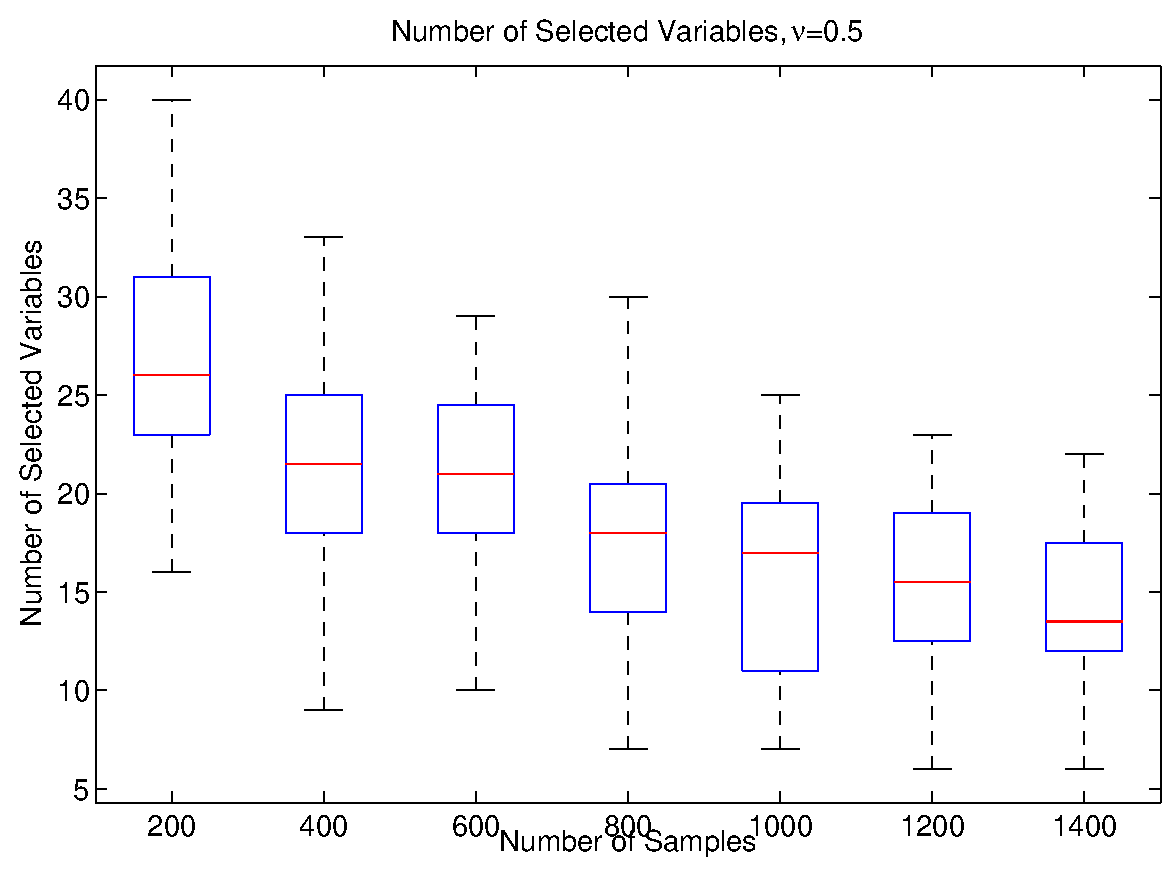
\includegraphics[width=.42\textwidth]{figs/C_support_box} & 
\includegraphics[width=.42\textwidth]{figs/CurveS}\\
(e) recovered support size & (f) nonparametric function
\end{tabular}
\end{center}
\caption{Support recovery results where the additive assumption is
  correct (a), incorrect (b), (c), and with correlated design (d).}\label{Support}
\vskip10pt
\end{figure*}



\subsection{Boston housing data}

We next use the Boston housing data rather than simulated data. This data set
contains 13 covariates, 506 samples and one response variable
indicating housing values in suburbs of Boston. The data and detailed description
can be found on the UCI Machine Learning Repository website\footnote{\url{http://archive.ics.uci.edu/ml/datasets/Housing}}. 

We first use all $n=506$ samples (with standardization) in the AC/DC algorithm,
using a set of candidate regularization parameters $\{\lambda^{(t)}\}$
ranging from $\lambda^{(1)} = 0$ (no regularization) to $2$. For each $\lambda^{(t)}$
we obtain a function value matrix $\bds{f}^{(t)}$ with $p=13$
columns and $n=506$ rows. The non-zero columns in this matrix indicate the variables selected using $\lambda^{(t)}$.  

In Figure~\ref{Boston}(a), we plot on the y-axis the norm $\|\bds{f}^{(t)}_j\|_{\infty}$ of every column $j$ against the regularization strength $\lambda^{(t)}$. Instead of plotting the value of $\lambda^{(t)}$ on the x-axis however, we plot the total norm at $\lambda^{(t)}$ normalized against the total norm at $\lambda^{(1)}$: $\frac{\sum_j \|\bds{f}^{(t)}_j\|_{\infty}}{\sum_j \|\bds{f}^{(1)}\|_{\infty}}$. Thus, as x-axis moves from 0 to 1, the regularization goes from strong to weak. For comparison, we
plot the LASSO/LARS result in a similar way in Figure \ref{Boston}(b).
From the figures we observe that the first three variables selected by
AC/DC and LASSO are the same: \tts{LSTAT}, \tts{RM} and \tts{PTRATIO},
consistent with previous findings~\citep{SpAM:07}.  The fourth
variable selected by AC/DC is \tts{INDUS} (with $\lambda^{(t)}=0.7$).
We then refit AC/DC with only these four variables without
regularization, and plot the estimated additive functions in Figure
\ref{Boston}(d). When refitting, we constrain a component to be convex if it is non-zero in the AC stage and concave if it is non-zero in the DC stage. As can be seen, these functions contain clear
nonlinear effects which cannot be captured by LASSO. The shapes of
these functions, including the concave shape of the \tts{PTRATIO} function, are in agreement with those obtained by
SpAM~\citep{SpAM:07}. 

Next, in order to quantitatively study the predictive performance, we
run 3 times 5-fold cross validation, following the same procedure
described above---training, variable selection and refitting.  A plot
of the mean and standard deviation of the predictive mean squared
error (MSE) is shown in Figure \ref{Boston}(c). Since for AC/DC the same
regularization level $\lambda^{(t)}$ may lead to a slightly different number of selected
variables in different folds and runs, the values on the $x$-axis
for AC/DC are not necessarily integers. The figure clearly shows that AC/DC has a 
lower predictive MSE than LASSO.  We also compared the performance of
AC/DC with that of Additive Forward Regression (AFR) presented
in~\cite{Xi:09}, and found that they are similar.  The main advantages
of AC/DC compared with AFR and SpAM are that there are no smoothing
parameters required, and the optimization is formulated
as a convex program, guaranteeing a global optimum.

%\begin{figure}[!htpb]
%        \centering
%        \begin{subfigure}[b]{0.45\textwidth}
%                \centering
%                \includegraphics[width=\textwidth]{figs/Additive}
%                 \caption{Variable selection result using AC/DC.}
%                \label{AC/DC}
%        \end{subfigure}
%        \begin{subfigure}[b]{0.45\textwidth}
%                \centering
%                \includegraphics[width=\textwidth]{figs/Additive1}
%                 \caption{Variable selection result using AC/DC.}
%                \label{AC/DC1}
%        \end{subfigure}\\
%        \begin{subfigure}[b]{0.45\textwidth}
%                \centering
%                \includegraphics[width=\textwidth]{figs/LASSO}
%                \caption{Variable selection result using LASSO.}
%                \label{LASSO}
%        \end{subfigure}
%        \begin{subfigure}[b]{0.45\textwidth}
%                \centering
%                \includegraphics[width=\textwidth]{figs/MSE}
%                 \caption{Predictive MSE of AC/DC and LASSO.}
%                 \label{MSE}
%        \end{subfigure}\\
%        \begin{subfigure}[b]{0.45\textwidth}
%                \centering
%                \includegraphics[width=\textwidth]{figs/Convex}
%                \caption{Inferred additive convex functions by AC/DC.}
%                \label{Convex}
%        \end{subfigure}
%        \caption{Results on Boston housing data.}\label{Boston}
%\end{figure}



\begin{figure*}
\begin{center}
\begin{tabular}{cc}
%\hskip-10pt
  \includegraphics[width=.38\textwidth]{figs/acdc_path}  &
%\hskip-25pt
  \includegraphics[width=.38\textwidth]{figs/lasso_path} 
\\
%\hskip-10pt 
(a) AC/DC $\|f_k\|_\infty$ paths & 
%\hskip-25pt
(b) LASSO $|\beta_k|$ paths \\
%\end{tabular}
%\begin{tabular}{cc}
  \includegraphics[width=.38\textwidth]{figs/MSEacdc} &
%\hskip 5pt
  \includegraphics[width=.45\textwidth]{figs/acdc_functs}
\\
(c) predictive MSE & (d) estimated functions from AC/DC
\end{tabular}
\end{center}
\caption{Results on Boston housing data, showing regularization paths,
 MSE and fitted functions.} \label{Boston}
\end{figure*}


% DO NOT CHANGE; RefTex variables -minx
 
%%% Local Variables: ***
%%% mode:latex ***
%%% TeX-master: "paper.tex" ***
%%% End: ***


\input{discussion}


\clearpage

%\bibliographystyle{plain}
\bibliography{local}

\newpage
\section{Appendix}
 
 
 \subsection{Proof of the Deterministic Condition for Sparsistency}
 \label{sec:deterministic_proof}
 
We restate Theorem~\ref{thm:deterministic} first for convenience. 
 
\begin{theorem} 
The following holds regardless of whether we impose the Lipschitz condition in optimization~\ref{opt:alternate_opt} and optimization~\ref{opt:alternate_opt_concave}.

Let $\{\hat{d}_k \}_{k \in S}$ be a minimizer of the restricted regression, that is, the solution to optimization (\ref{opt:alternate_opt}) where we restrict $k \in S$. 
Let $\hat{r} \coloneqq Y - \sum_{k \in S} \bar{\Delta}_k \hat{d}_k$ be the restricted regression residual. \\

Suppose for all $k\in S^c$, for all $i=1,...,n$, $\lambda_n > | \frac{1}{2n}
\hat{r}^\tran \mathbf{1}_{(i:n)}|$ where $\mathbf{1}_{(i:n)}$ is 1 on the coordinates of the $i$-th largest to the $n$-th largest entries of $X_k$ and 0 elsewhere.\\

Then the following are true:
\begin{enumerate}
\item Let $\hat{d}_k = 0$ for $k \in S^c$, then \{$\hat{d}_k\}_{k=1,...,p}$ is an optimal solution to optimization~\ref{opt:alternate_opt}. Furthermore, any solution to the optimization program \ref{opt:alternate_opt} must be zero on $S^c$.
\item For all $k \in S^c$, the solution to optimization~\ref{opt:alternate_opt_concave} must be 0 and must be unique.
\end{enumerate}
\end{theorem}


\begin{proof} 
We will omit the Lipschitz constraint in our proof here. It is easy to add that in and check that the result of the theorem still holds.\\

We first consider the first item in the conclusion of the theorem.

We will show that with $\{\hat{d}_k\}_{k=1,..,p}$ as constructed, we can set the dual variables to satisfy complementary slackness and stationary conditions: $\nabla_{d_k} \mathcal{L}(\hat{d})  = 0$ for all $k$.\\ 

The Lagrangian is
\begin{equation}
\label{eqn:full_lagrange}
\mathcal{L}( \{ d_k \}, \nu) = 
  \frac{1}{2n} \Big\| 
    Y - \sum_{k=1}^p  \bar{\Delta}_k d_k  \Big\|_2^2 + 
    \lambda \sum_{k=1}^p \| \bar{\Delta}_k d_k \|_\infty -
    \sum_{k=1}^p \sum_{i=2}^{n-1} \nu_{ki} d_{ki} 
\end{equation}
with the constraint that $\nu_{ki} \geq 0$ for all $k,i$.

Because $\{\hat{d}_k\}_{k \in S}$ is by definition the optimal solution of the restricted regression, it is a consequence that stationarity holds for $k \in S$, that is, $\partial_{ \{ d_k \}_{k \in S} } \mathcal{L}(d) = 0$, and that the dual variables $\nu_k$ for $k \in S$ satisfy complementary slackness.

We now verify that stationarity holds also for $k \in S^c$. We fix one dimension $k \in S^c$ and let $\hat{r} = Y - \sum_{k' \in S} \bar{\Delta}_{k'} \hat{d}_{k'}$. 

The Lagrangian form of the optimization, in term of just $d_k$, is
\[
\mathcal{L}(d_k, \nu_k) =
  \frac{1}{2n} \big\| Y - \sum_{k' \in S} \bar{\Delta}_{k'} d_{k'} 
  -  \bar{\Delta}_k d_k \big\|_2^2 
   + \lambda \| \bar{\Delta}_k d_k\|_\infty
  - \sum_{i=2}^{n-1} \nu_{ki} d_{ki}
\]
with the constraint that $v_i \geq 0$ for all $i$. 

The derivative of the Lagrangian is:
\begin{align*}
\partial_{d_k} \mathcal{L}(d_k) =  -\frac{1}{n} \bar{\Delta}_k^\tran ( Y - \sum_{k'\in S} \bar{\Delta}_{k'} d_{k'}  - \bar{\Delta}_k d_k )
        + \lambda \bar{\Delta}_k^\tran \mathbf{u}
      - \nu_k
\end{align*}
where $\mathbf{u}$ is the subgradient of $\| \bar{\Delta}_k d_k \|_\infty$, an $n$-vector such that $\| \mathbf{u}_T \|_1 = 1$ where $T = \{ i \,:\,  (\bar{\Delta}_k d_k)_i = \| \bar{\Delta}_k d_k \|_\infty \}$.

We now substitute in $d_{k'} = \hat{d}_{k'}$ for $k' \in S$, $d_k = 0$ for $k \in S$, and $r = \hat{r}$ and show that the duals can be set in a way to ensure that the derivatives are equal to 0.

\begin{align*}
\partial_{d_k} \mathcal{L}(\hat{d}_k) = -\frac{1}{n} \bar{\Delta}_k^\tran\hat{r} + \lambda \bar{\Delta}_k^\tran \mathbf{u}
           - \nu_k = 0 
\end{align*}
where $\| \mathbf{u} \| \leq 1$ and $\nu_k \geq 0$. It clear that to show stationarity, we only need to show that $-\frac{1}{n} \bar{\Delta}_k^\tran \hat{r} + \lambda \bar{\Delta}_k^\tran \mathbf{u} \geq 0$ hwere the inequality is element-wise.

Let us reorder the samples so that the $i$-th sample is the $i$-smallest sample. \\

We will construct $\gamma = 0$, and $\mathbf{u} = (-a, 0, ..., a)$ for some $0 < a < 1/2$. (coordinates of $\mathbf{u}$ correspond to the new sample ordering) We then just need to show that
\begin{align*}
- \frac{1}{n} \bar{\Delta}_k^\tran \hat{r} + \lambda \bar{\Delta}_k^\tran \mathbf{u} &\geq 0 \quad \Leftrightarrow \\
- \frac{1}{n} \Delta_k^\tran \hat{r} + \lambda \Delta_k^\tran \mathbf{u} &\geq 0 \quad \Leftrightarrow\\
- \frac{1}{n} \sum_{i > j} (X_{ki} - X_{kj}) \hat{r}_i + \lambda (X_{kn} - X_{kj})a &\geq 0 \quad 
   \textrm{for each } j \\
- \frac{1}{n} \sum_{i > j} \sum_{j < i' \leq i} \mathsf{gap}_{i'} \hat{r}_i 
    + \lambda (X_{kn} - X_{kj})a &\geq 0 \\
- \frac{1}{n} \sum_{i' > j} \mathsf{gap}_{i'} \sum_{i \geq i'} \hat{r}_i 
    + \lambda (X_{kn} - X_{kj})a &\geq 0 \\
- \frac{1}{n} \sum_{i' > j} \mathsf{gap}_{i'} \mathbf{1}_{(i':n)}^\tran \hat{r} 
   + \lambda (X_{kn} - X_{kj})a &\geq 0 
\end{align*}
where $\mathsf{gap}_i = X_{ki} - X_{k,i-1}$. If $\frac{1}{2n} |\mathbf{1}_{(i:n)}^\tran \hat{r}| \leq \lambda a$ for all $i=1,...,n$, then we have that:

\begin{align*}
- \frac{1}{n} \sum_{i' > j} \mathsf{gap}_{i'} \mathbf{1}_{i':n}^\tran \hat{r}
   + \lambda (X_{kn} - X_{kj})a &\geq 0 \quad \Leftrightarrow \\
- \sum_{i' > j} \mathsf{gap}_{i'} \lambda a + \lambda (X_{kn} - X_{kj}) a &\geq 0\\
- (X_{kn} - X_{kj}) \lambda a + \lambda (X_{kn} - X_{kj}) a &\geq 0
\end{align*}

We have thus proven that there exist one solution $\{ \hat{d}_k \}_{k=1,...,p}$ such that $\hat{d}_k = 0$ for all $k \in S^c$. Furthermore, we have shown that the subgradient variables $\mathbf{u}_k$ of the solution $\{ \hat{d}_k \}$ can be chosen such that $\| \mathbf{u}_k \|_1 < 1$ for all $k \in S^c$.  We now prove that if $\{ \hat{d}'_k \}_{k = 1,..., p}$ is another solution, then it must be that $\hat{d}'_k = 0$ for all $k \in S^c$ as well.  \\

%% prove uniqueness of sparsity pattern.

We first claim that $\sum_{k=1}^p \bar{\Delta}_k \hat{d}_k = \sum_{k=1}^p \bar{\Delta}_k \hat{d}'_k$. If this were not true, then a convex combination of $\hat{d}_k, \hat{d}'_k$ would achieve a strictly lower objective on the quadratic term. More precisely, let $\zeta \in [0,1]$. If $\sum_{k=1}^p \bar{\Delta}_k \hat{d}'_k \neq \sum_{k=1}^p \bar{\Delta}_k \hat{d}_k$, then $\| Y - \sum_{k=1}^p \bar{\Delta}_k \big( \hat{d}_k + \zeta ( \hat{d}'_k - \hat{d}_k) \big) \|_2^2$ is strongly convex as a function of $\nu$. Thus, it cannot be that $\hat{d}_k$ and $\hat{d}'_k$ both achieve optimal objective and we have reached a contradiction.\\

Now, we look at the stationarity condition for both $\{ \hat{d}_k \}$ and $\{ \hat{d}'_k \}$. Let $\mathbf{u}_k \in \partial \| \bar{\Delta}_k \hat{d}_k \|_\infty$ and let $\mathbf{u}'_k \in \partial \| \bar{\Delta}_k \hat{d}'_k \|_\infty$ be the two sets of subgradients. Let $\{ \nu_{ki} \}_{k=1,..,p,\, i=1,...n-1}$ and $\{ \nu'_{ki} \}$ be the two sets of positivity dual variables. \footnote{since there is no positivity constraint on $d_{k1}$, we let $\nu_{k1} = 0$ always.}

Let us define $\bar{\Delta}$, a $n \times p(n-1)$ matrix, to denote the column-wise concatenation of $\{ \bar{\Delta}_k \}_k$ and $\hat{d}$, a $p(n-1)$ dimensional vector, to denote the concatenation of $\{ \hat{d}_k \}_k$. With this notation, we can express $\sum_{k=1}^p \bar{\Delta}_k \hat{d}_k = \bar{\Delta} \hat{d}$.

Since both solutions $(\hat{d}, \mathbf{u}, \nu)$ and $(\hat{d}', \mathbf{u}', \nu')$ must satisfy the stationarity condition, we have that:
\[
\bar{\Delta}^\tran ( Y - \bar{\Delta} \hat{d} ) 
   + \lambda \sum_{k=1}^p \bar{\Delta}_k^\tran \mathbf{u}_k - \nu = 
\bar{\Delta}^\tran ( Y - \bar{\Delta} \hat{d}' ) 
   + \lambda \sum_{k=1}^p \bar{\Delta}_k^\tran \mathbf{u}'_k - \nu' = 0
\] 
We multiply both sides of the above equation by $\hat{d}'$:
\[
\hat{d}'^{\tran}  \bar{\Delta}^\tran ( Y - \bar{\Delta} \hat{d} ) 
    + \lambda \sum_{k=1}^p \hat{d}'^\tran_k \bar{\Delta}_k^\tran \mathbf{u}_k - \hat{d}'^\tran \nu = \hat{d}'^{\tran}  \bar{\Delta}^\tran ( Y - \bar{\Delta} \hat{d}' ) 
    + \lambda \sum_{k=1}^p \hat{d}'^\tran_k \bar{\Delta}_k^\tran \mathbf{u}'_k - \hat{d}'^\tran \nu'
\]
Since $\bar{\Delta} \hat{d}_k = \bar{\Delta} \hat{d}$, $\hat{d}'^\tran \nu' = 0$ (complementary slackness), and $\hat{d}'^\tran_k \bar{\Delta}_k^\tran \mathbf{u}'_k  = \| \hat{f}'_k \|_\infty$ (where $\hat{f}'_k = \bar{\Delta}_k \hat{d}'_k$), we have that:
\[
\lambda \sum_{k=1}^p \hat{d}'^\tran_k \bar{\Delta}_k^\tran \mathbf{u}_k - \hat{d}'^\tran \nu = \lambda \sum_{k=1}^p \| \hat{f}'_k \|_\infty
\]
On one hand, $\hat{d}'$ is a feasible solution so $\hat{d}'^\tran \nu \geq 0$ and so 
\[
\sum_{k=1}^p \hat{d}'^\tran_k \bar{\Delta}_k^\tran \mathbf{u}_k \geq \sum_{k=1}^p \| \hat{f}'_k \|_\infty .
\]

On the other hand, by Holder's inequality:
\begin{align*}
\sum_{k=1}^p \hat{d}'^\tran_k \bar{\Delta}_k^\tran \mathbf{u}_k &\leq 
   \sum_{k=1}^p \| \hat{f}'_k \|_\infty \|\mathbf{u}_k \|_1 
\end{align*}

Since $\mathbf{u}_k$ can be chosen so that $\| \mathbf{u}_k \|_1 < 1$ for all $k \in S^c$, we would get a contradiction if $\| \hat{f}'_k \|_\infty > 0$ for some $k \in S^c$. We thus conclude that $\hat{d}'$ must follow the same sparsity pattern.\\


The second item in the theorem concerning optimization~\ref{opt:alternate_opt_concave} is proven in exactly the same way. 

The Lagrangian of optimization~\ref{opt:alternate_opt_concave} is:
\[
\mathcal{L}_{\trm{cave}}(d_k, \nu_k) = 
  \frac{1}{2n} \big\| \hat{r} - \bar{\Delta}_k d_k \big \|_2^2 + 
  \lambda \| \bar{\Delta}_k d_k \|_\infty + \sum_{k=1}^p \sum_{i=2}^{n-1} \nu_{ki} d_{ki}
\]

The exact same reasoning applies to show that $\hat{d}_k = 0$ satisfies KKT conditions sufficient for optimality.

\end{proof}
 
 
 
 
 
 
 \subsection{Proof of False Positive Control}
 \label{sec:false_positive_proof}
 
\textbf{Note:} the symbols $c,C$ represent absolute constants. We will often abuse notation and ``absorb'' new absolute constants into $c, C$; the actual value of $c, C$ could thus vary from line to line.

 We first restate the theorem for convenience. 
 

\begin{theorem} 
Suppose assumptions A1-A4 hold. 

Suppose $\lambda_n \geq c s Lb \sigma  \sqrt{ \frac{1}{n} \log^2 np}$, then with probability at least $ 1 - \frac{C}{n}$, for all $k \in S^c$, and for all $i'=1,...,n$:
\[
\lambda_n > \Big| \frac{1}{2n}\hat{r}^\tran \mathbf{1}_{(i':n)} \Big|
\]

And therefore,for all $k \in S^c$, both the AC solution $\hat{f}_k$, from optimization~\ref{opt:alternate_opt}, and the DC solution $\hat{g}_k$, from optimization~\ref{opt:alternate_opt_concave} are zero. 
\end{theorem}

\begin{proof}
The key is to note that $\hat{r}$ and $\Delta_{k,j}$ are independent for all $k \in S^c,j=1,...,n$ because $\hat{r}$ is only dependent on $X_{S}$.

Fix $j$ and $i$. $\hat{r}^\tran \mathbf{1}_{(i':n)}$ is then the sum of $n-i'+1$ random coordinates of $\hat{r}$. We will then use Serfling's theorem on the concentration of measure of sampling without replacement. (corollary~\ref{cor:serfling}) We must first bound $\| \hat{r} \|_\infty$ and $\frac{1}{n} \sum_{i=1}^n \hat{r}_i$ before we can use Serfling's results however.\\

\textbf{Step 1}: Bounding $\| \hat{r} \|_\infty$. 

$\hat{r}_i = f_0(x_i) + w_i - \hat{f}(x_i)$ where $\hat{f}(x_i) = \sum_{k \in S} \bar{\Delta}_k \hat{d}_k$ is the convex additive function outputted by the restricted regression.

Both $f_0(x_i)$ and $\hat{f}(x_i)$ are coordinate-wise $L$-Lipschitz and therefore are bounded by $2 sLb$. 

Because $w_i$ is subgaussian, $|w_i| \leq c \sigma \sqrt{\log \frac{2}{\delta}}$ with probability at most $1-\delta$. By union bound across $i=1,...,n$, we have that $\| w\|_\infty \leq c \sigma \sqrt{ \log \frac{2}{\delta}}$ with probability at most $1 - n \delta$.

We now put this together and take another union bound across all $j$ and all $i'$:
\begin{align*}
\| \hat{r} \|_\infty &\leq c (sLb + \sigma \sqrt{ \log \frac{2}{\delta}}) \\
      &\leq c sLb \sigma \sqrt{\log \frac{2}{\delta}}
\end{align*}
with probability at least $1 - n^2 p \delta$. We supposed that both $sLb \geq 2$ and $\sigma\sqrt{\log \frac{2}{\delta}} \geq 2$.

\textbf{Step 2}: Bounding $| \frac{1}{n} \hat{r}^\tran \mathbf{1} |$. 

\begin{align*}
\frac{1}{n} \hat{r}^\tran \mathbf{1} &= 
    \frac{1}{n} \sum_{i=1}^n f_0(x_i) + w_i - \hat{f}(x_i) \\
  &= \frac{1}{n} \sum_{i=1}^n f_0(x_i) + w_i \quad \trm{ ($\hat{f}$ is centered)}
\end{align*}

Because $|f_0(x_i)| \leq sLb$, the first term $| \frac{1}{n} \sum_{i=1}^n f_0(x_i)|$ is at most $2 sLb \sqrt{\frac{1}{n} \log \frac{2}{\delta}}$ with probability at most $1-\delta$ by Hoeffding Inequality.

Because $w_i$ is subgaussian, the second term $|\frac{1}{n} \sum_{i=1}^n w_i|$ is at most $2 \sigma \sqrt{ \frac{1}{n} \log \frac{2}{\delta}}$ with probability at most $1-\delta$.

Taking an union bound, we have that 

\begin{align*}
| \frac{1}{n} \hat{r}^\tran \mathbf{1}| &\leq 2 sLb \sqrt{\frac{1}{n} \log \frac{2}{\delta}} + 2 \sigma \sqrt{\frac{1}{n} \log \frac{2}{\delta}} \\
  &\leq c sLb \sigma \sqrt{\frac{1}{n} \log \frac{2}{\delta}} 
\end{align*}
with probability at least $1-2\delta$.\\

\textbf{Step 3}: We now apply Serfling's theorem.

Serfling's theorem states that with probability at least $1 - \delta$:
\[
\Big
|\frac{1}{n} \hat{r}^\tran \mathbf{1}_{(i':n)}\Big| \leq
   2\| \hat{r} \|_\infty \sqrt{ \frac{1}{n} \log \frac{2}{\delta}} + 
   \Big|\frac{1}{n} \hat{r}^\tran \mathbf{1} \Big|
\]

Taking an union bound across previous events, we have that with probability at least $1 - 3n^2 p \delta$, for all $j \in S^c$, for all $i'=1,...,n$:
\begin{align*}
\Big|\frac{1}{n} \hat{r}^\tran \mathbf{1}_{(i':n)} \Big| &\leq
  c sLb \sigma \sqrt{\frac{1}{n} \log \frac{2}{\delta}} 
\end{align*}
Setting $\delta = \frac{1}{n^3 p}$ gives the desired result.

\end{proof}

 
 
%%%%%%%%%%%%%%%%%%%%%%%%%%%%%%
%%
%%
%%
%%
%%%%%%%%%%%%%%%%%%%%%%%%%%%%%% 
 
 \subsection{Proof of False Negative Control}
 \label{sec:false_negative_proof}
 
\textbf{Note:} the symbols $c,C$ represent absolute constants. We will often abuse notation and ``absorb'' new absolute constants into $c, C$; the actual value of $c, C$ could thus vary from line to line.

 We first introduce notations.
 \subsubsection{Notation} 
\label{sec:false_negative_proof_notations}

Let $f : \mathbb{R}^s \rightarrow \R$, we denote $\| f \|_P \equiv \E f(X)^2$. \\
Given samples $X_1,...,X_n$, we denote $\| f \|_n \equiv \frac{1}{n} \sum_{i=1}^n f(X_i)^2$ and $\langle f, g \rangle_n \equiv \frac{1}{n} \sum_{i=1}^n f(X_i) g(X_i)$. \\

Let $\mathcal{C}^1$ denote the set of univariate convex functions supported on $[-b,b]$. Let $\mathcal{C}^1_L \equiv \{ f \in \mathcal{C}^1 \,:\, \| \partial f \|_\infty \leq L \}$ denote the set of $L$-Lipschitz univariate convex functions. \\

Define $\mathcal{C}^s$ as the set of convex additive functions and $\mathcal{C}^s_L$ likewise as the set of $L$-Lipschitz convex additive functions.
\begin{align*}
\mathcal{C}^s &\equiv \{ f \,:\, f = \sum_{k=1}^s f_k, \,
   f_k \in \mathcal{C}^1 \} \\
\mathcal{C}^s_L &\equiv \{ f \in \mathcal{C}^s \,:\, 
f = \sum_{k=1}^s f_k, \, \| \partial f_k \|_\infty \leq L \}
\end{align*}

Let $f^*(x) = \sum_{k=1}^s f^*_k(x_k)$ be the population risk minimizer:
\[
f^* = \arg\min_{f \in \mathcal{C}^s} \| f_0 - f^* \|_P^2
\]

We let $L$ be an upper bound on $\| \partial_{x_k} f_0 \|_\infty$ and $\| \partial f^*_k \|_\infty$. Since $f_0, f^*$ are supported on $[-b, b]^s$, it follows that $\| f_0 \|_\infty, \|f^* \|_\infty \leq s L b$.

We define $\hat{f}$ as the empirical risk minimizer:
\[
\hat{f} = \arg\min \Big \{ \| y - f \|_n^2 + \lambda \sum_{k=1}^s \| f_k \|_\infty 
    \,:\, f \in \mathcal{C}^s_L, \mathbf{1}_n^\tran f_k = 0 \Big \}
\]

For $k \in \{1,...,s\}$, define $g^*_k$ to be decoupled concave population risk minimizer
\[
g^*_k \equiv \argmin_{g_k \in \mh \mathcal{C}^1} \| f_0 - f^* - g_k \|_P^2 
\]
In our proof, we will analyze $g^*_k$ for $k$'s such that $f^*_k = 0$. Likewise, we define the empirical version:
\[
\hat{g}_k \equiv \argmin \Big\{ \| f_0 - \hat{f} - g_k \|_n^2 \,:\, g_k \in \mh \mathcal{C}^1_L \,, \mathbf{1}_n^\tran g_k = 0 \Big\}
\]
By the definition of the ACDC procedure, $\hat{g}_k$ exist only for $k$ that have zero in their convex additive approximation.


\subsubsection{Proof}
 
By additive faithfulness of the ACDC procedure, it is necessary that $f^*_k \neq 0$ or $g^*_k \neq 0$ for all $k \in S$. \\


Intuitively, we would like to show the following:
\begin{align*}
\| f_0 - \hat{f} \|_P & \approx \| f_0 - f^* \|_P \\
\| f_0 - f^* - \hat{g}_k \|_P & \approx \| f_0 - f^* - g^*_k \|_P 
       \quad \trm{for all $k \in S$ where $f^*_k = 0$}
\end{align*}
where the estimation error is a term that decreases with $n$.

Suppose $\hat{f}_k = 0$ and $f^*_k \neq 0$, then, when $n$ is large enough, there must exist a contradiction because the population risk of $f^*$, $\| f_0 - f^* \|_P$, is strictly larger than the population risk of the best approximation whose $k$-th component is constrained to be zero. 

Suppose $f^*_k = 0$, then $g^*_k \neq 0$. When $n$ is large enough, $\hat{g}_k$ must not be zero or we would have another contradiction. \\


\begin{theorem}
\label{thm:convex_consistent}
Let $\hat{f}$ be the minimizer of the restricted regression with $\lambda \leq sB \sqrt{ \frac{1}{n} \log^2 np}$.

Suppose $n \geq c_1 \max(\sqrt{sB}, B)$ and $\sigma \geq c_2$ for some constant $c_1, c_2 > 0$.

Then, with probability at least $1-\delta$,
\begin{align}
\|f_0 - \hat{f} \|_P^2 - \| f_0 - f^* \|_P^2 
&\leq c B^3\sigma \sqrt{ \frac{s^5}{n^{4/5}} \log^2 \frac{Cnp}{\delta}}
\end{align}
Where $c, C$ are constants, dependent on $c_1, c_2$.

\end{theorem}


\begin{proof}

\textbf{Step 1.} We start from the definition. 

\begin{align*}
\| y - \hat{f} \|_n^2 + \lambda \sum_{k=1}^s \| \hat{f}_k \|_\infty &\leq
  \| y - f^* + \bar{f}^* \|_n^2 + \lambda \sum_{k=1}^s \| f^*_k - \bar{f}^* \|_\infty 
\end{align*}
We plug in $y = f_0 + w$:
\begin{align*}
\| f_0 + w - \hat{f} \|_n^2 + \lambda \sum_{k=1}^s \Big( \| \hat{f}_k \|_\infty - 
    \| f^*_k - \bar{f}^*_k \|_\infty \Big) &\leq \|f_0 + w - f^* + \bar{f}^* \|_n^2 \\
\| f_0 - \hat{f} \|_n^2 + 2\langle w, f_0 - \hat{f} \rangle_n 
     +\lambda \sum_{k=1}^s \Big( \| \hat{f}_k \|_\infty - \|f^*_k -\bar{f}^*_k\|_\infty \Big) 
    &\leq \| f_0 - f^* + \bar{f}^* \|_n^2 + 
    2 \langle w, f_0 - f^* + \bar{f}^* \rangle \\
\|f_0 - \hat{f} \|_n^2 - \| f_0 - f^* + \bar{f}^* \|_n^2 + 
    \lambda \sum_{k=1}^s \Big( \| \hat{f}_k \|_\infty - 
 \| f^*_k - \bar{f}^*_k \|_\infty \Big) &\leq 2 \langle w, \hat{f} - f^* + \bar{f}^* \rangle
\end{align*}

The middle term can be bounded with the fact that $\|f^*_k - \bar{f}^*_k \|_\infty \leq 4B$.

\begin{align*}
\|f_0 - \hat{f} \|_n^2 - \| f_0 - f^* + \bar{f}^* \|_n^2 
   &\leq 2 \langle w, \hat{f} - f^* + \bar{f}^* \rangle + \lambda 4 s B 
\end{align*}

Using Lemma~\ref{lem:remove_centering}, we can remove $\bar{f}^*$ from the LHS. With probability at least $1 - \delta$:
\begin{align}
\label{eqn:first_step_inequality}
\|f_0 - \hat{f} \|_n^2 - \| f_0 - f^* \|_n^2 
   &\leq 2 \langle w, \hat{f} - f^* + \bar{f}^* \rangle + \lambda 4 s B + c(sB)^2 \frac{1}{n} \log \frac{2}{\delta}
\end{align}

%[TOOD: at this point, we still have to choose a value for $\lambda$]\\

%%%%%%%%%%%%%%%%%%%%%%%%%%%%%%
%% 
%% Step 2
%%
%%
%%%%%%%%%%%%%%%%%%%%%%%%%%%%%%

\textbf{Step 2.} We upper bound $2 \langle w, \hat{f} - f^* + \bar{f}^* \rangle$ with bracketing entropy.

Define $\mathcal{G}$ as $\{ f - f^* + \bar{f}^* \,:\, f \in \mathcal{C}^s\}$ as the set of convex additive functions centered around the function $f^* - \bar{f}^*$. 

By Corollary~\ref{prop:convexbracket_lp}, there is an $\epsilon$-bracketing of $\mathcal{G}$ whose size is bounded by $\log N_{[]}( 2\epsilon, \mathcal{G}, L_1(P)) \leq sK^{**} \left( \frac{2sbB}{\epsilon} \right)^{1/2}$, for all $\epsilon \in (0, sB \epsilon_3]$.

By Corollary~\ref{cor:convexbracket_ln}, with probability at least $1-\delta$, each bracketing pair $(h_U, h_L)$ is close in $L_1(P_n)$ norm, i.e., for all $(h_U, h_L)$, 
$\frac{1}{n} \sum_{i=1}^n | h_U(X_i) - h_L(X_i) | \leq 2 \epsilon + sB \sqrt{ \frac{sK^{**}(2sbB
)^{1/2} + \log \frac{1}{\delta}}{2\epsilon^{1/2} n}}$.

For each $h \in \mathcal{G}$, there exists a pair $(h_U, h_L)$ such that $h_U(X_i) - h_L(X_i) \geq h(X_i) - h_L(X_i) \geq 0$. Therefore, with probability at least $1-\delta$, uniformly for all $h \in \mathcal{G}$:

$$
\frac{1}{n} \sum_{i=1}^n |h(X_i) - h_L(X_i)| \leq \frac{1}{n} \sum_{i=1}^n | h_U(X_i) - h_L(X_i)| \leq 2\epsilon +  (sB) \sqrt{ \frac{sK^{**}(2sbB)^{1/2} \log \frac{1}{\delta}}{2\epsilon^{1/2} n}}
$$.
Where we assumed that condition~\ref{cond:simplify_covering_number} holds. 

We denote $\epsilon_{n,\delta} \equiv (sB) \sqrt{ \frac{sK^{**}(2sbBc_u)^{1/2} \log \frac{1}{\delta}}{2\epsilon^{1/2} n}}$. 
Therefore,  
\[
|\langle w, h - h_L\rangle_n| \leq \| w \|_\infty \frac{1}{n} \sum_{i=1}^n |h(X_i) - h_L(X_i)| \leq
  \sigma \sqrt{\log \frac{n}{\delta}} \left( \epsilon + \epsilon_{n,\delta} \right)
\]
For the last inequality, we used the fact that $w$ is a vector of independent subgaussian($\sigma$) random variables and hence, by union bound, with probability at least $1-\delta$, $\| w \|_\infty \leq \sigma \sqrt{\log \frac{n}{\delta}}$. 

By another property of subgaussian random variables, with probability at least $1-\delta$, $|\langle w, h_L \rangle_n | \leq \| h_L \|_n \sigma \sqrt{ \frac{1}{cn} \log \frac{1}{\delta} }$. Applying an union bound, we have that 
$\sup_{h_L} |\langle w, h_L \rangle| \leq sB \sigma \sqrt{ \frac{\log N_{[]}}{n} \log \frac{1}{\delta}}$.

Putting this together, we have that
\begin{align*}
|\langle w, h \rangle_n | &\leq | \langle w, h_L\rangle_n| + |\langle w, h - h_L\rangle_n|\\
|\sup_{h \in \mathcal{G}} \langle w, h \rangle_n| &\leq 
     | \sup_{h^L} \langle w, h^L \rangle_n | + \sigma \sqrt{\log \frac{n}{\delta}} (\epsilon + \epsilon_{n, \delta}) \\
   &\leq   sB \sigma \sqrt{ \frac{ \log N_{[]} + \log \frac{1}{\delta}}{cn}} + \sigma \sqrt{\log \frac{n}{\delta}} (\epsilon + \epsilon_{n, \delta}) \\
   &\leq  sB \sigma \sqrt{ \frac{sK^{**} (2sbB)^{1/2} \log \frac{1}{\delta}}{cn \epsilon^{1/2}}} +
   \sigma \sqrt{ \log \frac{n}{\delta}} (\epsilon + \epsilon_{n, \delta}) \\
   &\leq sB \sigma \sqrt{ \frac{sK^{**} (2sbB)^{1/2} \log \frac{1}{\delta}}{cn \epsilon^{1/2}}} +
   \sigma\sqrt{\log \frac{n}{\delta}} \epsilon + sB \sigma \sqrt{ \frac{sK^{**} (2sbB)^{1/2} + \log \frac{1}{\delta}}{cn \epsilon^{1/2}} \log \frac{n}{\delta}} \\
   &\leq \sigma\sqrt{\log \frac{n}{\delta}} \epsilon + sB \sigma \sqrt{ \frac{sK^{**} (2sbB)^{1/2} \log^2 \frac{n}{\delta}}{cn \epsilon^{1/2}}} \\
\end{align*}

The two terms are balanced when one sets $\epsilon = sB \sqrt{ \frac{(s K^{**} (sBb)^{1/2})^{4/5}}{n^{4/5}} }$.  

This is only valid if $n$ is large enough so that $\epsilon \in (0, sB \epsilon_3]$.

Also, to ensure that conditions~\ref{cond:simplify_covering_number} hold, we need that $\log n \geq 2$ and $n \geq c B$ where $c$ is some constant dependent only on $K^{**}$ and $b$.

We upper bound some terms to simplify the presentations again and end up with the following result:

\[
|\sup_{h \in \mathcal{G}} \langle w, h \rangle | \leq sB \sigma \sqrt{ 
   \frac{s b^{1/2} \log^2 \frac{n}{\delta}}{c n^{4/5}}}
\]

% Then, $\| h \|_n \leq \| h \|_\infty \leq 4sLb$ for all $h \in \mathcal{G}$.\\

% According to theorem~\ref{thm:chaining}, for all $\epsilon > \frac{1}{\sqrt{n}}\sigma c \int_0^R \sqrt{ \log N_2(t, \mathcal{G}) }dt \vee R$,
% \[
% P\Big( \sup_{h \in \mathcal{G}} \langle w, h \rangle_n \geq \epsilon \Big) \leq
%   4 \exp \Big( - \frac{ n \epsilon^2}{ c R^2 \sigma^2} \Big)
% \]
% where $R = 4sLb$ for our purpose.

% Restated, we have that, with probablity at least $1-\delta$,
% \[
% \sup_{h \in \mathcal{G}} | \langle w, h \rangle_n | \leq 
%    c R \sigma \sqrt{ \frac{1}{n} \log \frac{4}{\delta}} + 
%       \Big( \int_0^R \sqrt{\log N_2(t, \mathcal{G})}dt \vee R \Big)\, 
%        c \sigma \sqrt{\frac{1}{n}} 
% \]

% Now we evaluate the integral. Since $N_{\|\cdot\|_n}(t, \mathcal{G}) \leq N_\infty(t, \mathcal{G})$, we know that $\sqrt{\log N_{\|\cdot\|_n}(t, \mathcal{G})} \leq \sqrt{C s^{1.5} b L} t^{-1/4}$.

% \begin{align*}
% \int_0^R \sqrt{\log N_{\|\cdot\|_n}(t, \mathcal{G})} dt &\leq 
%       \sqrt{C s^{1.5} b L} \int_0^R t^{-1/4} dt \\ 
%  &= \sqrt{C s^{1.5} b L} \, \frac{4}{3} R^{3/4} \\
%  &= \sqrt{C s^{1.5} b L} \, c (sLb)^{3/4} \\
%  &\leq c (s b L)^2
% \end{align*}

% Coming back, we have, with probability at least $1-\delta$,
% \begin{align*}
% \sup_{h \in \mathcal{G}} | \langle w, h \rangle | &\leq 
%    c sLb \sigma \sqrt{ \frac{1}{n} \log \frac{4}{\delta} } + 
%     c (sLb)^2 \sigma \sqrt{ \frac{1}{n} } \\
%  &\leq c (sLb)^2\sigma \sqrt{ \frac{1}{n} \log \frac{4}{\delta} }
% \end{align*}


Plugging this result into equation~\ref{eqn:first_step_inequality} and using an union bound, we get, with probability at least $1 - 2\delta$:
\begin{align}
\|f_0 - \hat{f} \|_n^2 - \| f_0 - f^* \|_n^2 
   &\leq c sB \sigma \sqrt{ 
   \frac{s b^{1/2} \log^2 \frac{n}{\delta}}{n^{4/5}}}
   + \lambda 4 s B + c (sB)^2 \frac{1}{n} \log \frac{2}{\delta} \nonumber\\
\|f_0 - \hat{f} \|_n^2 - \| f_0 - f^* \|_n^2 
   &\leq c sB \sigma \sqrt{ 
   \frac{s b^{1/2} \log^2 \frac{nC}{\delta}}{n^{4/5}}}
   + \lambda 4 s B \nonumber\\   
   &\leq c B \sigma 
    \sqrt{ \frac{s^3 b^{1/2}}{n^{4/5}} \log^2 \frac{n}{\delta}} + \lambda 4 sB
\label{eqn:second_step_inequality}
\end{align}

%%%%%%%%%%%%%%%%%%%%%%%%%%%%%%
%%
%% Step 3.
%%
%%
%%%%%%%%%%%%%%%%%%%%%%%%%%%%%%

\textbf{Step 3.} We continue from equation~\ref{eqn:second_step_inequality}, use lemma~\ref{lem:uniform_convergence}, use another union bound, with probability at least $1-3\delta$,

\begin{align}
\|f_0 - \hat{f} \|_P^2 - \| f_0 - f^* \|_P^2 
   &\leq cB^2 \sigma 
    \sqrt{ \frac{s^3 b^{2/5}}{n^{4/5}} \log^2 \frac{Cn}{\delta}}
 +\lambda 4 s B + c B^3 \sqrt{ \frac{s^5}{n^{4/5}} \log \frac{2}{\delta}}
    \nonumber \\
&\leq c B^3 \sigma \sqrt{ \frac{s^5 b^{2/5}}{n^{4/5}} \log^2 \frac{Cn}{\delta}} + \lambda 4 sB \nonumber
\end{align}
Where for the second inequality, we used the assumption that there is some large constant $c$ such that $B \geq \frac{\sigma}{c\sigma + 1}$.

Substituting in $\lambda \leq c sB \sqrt{\frac{1}{n} \log^2 np}$ and we get the desired result.

\end{proof}
 
%% End of "No False Negative" proof for the f's






\begin{theorem}
\label{thm:concave_consistent}
Let $\hat{g}_k$ denote the minimizer of the concave postprocessing with $\lambda \leq c sB \sqrt{\frac{1}{n} \log^2 np}$.\\

Suppose $n$ is large enough such that $B^3 \sigma \sqrt{ \frac{s^5}{n^{4/5}} \log^2 \frac{4np}{\delta} } \leq 1$.\\

Then, with probability at least $1- s\delta$, for all $k=1,...,s$:\\
\[
\| f_0 - f^* - \hat{g}_k \|_P^2 - \| f_0 - f^* - g^*_k \|_P^2 \leq  c (Lb)^{2.5} \sigma^{0.5} \sqrt[4]{ \frac{s^5}{n^{4/5}} \log^2 \frac{4np}{\delta}} 
\]
\end{theorem}

\begin{proof}
The proof proceeds almost identically to that of theorem~\ref{thm:convex_consistent} because convex and concave functions have the same bracketing number.

\textbf{Step 1.} We start from the definition of $\hat{g}_k$:
\begin{align*}
\| y - \hat{f} - \hat{g}_k \|_n^2 + \lambda \| \hat{g} \|_\infty &\leq
   \| y - \hat{f} - g^*_k \|_n^2 + \lambda \| g^* \|_\infty \\
\| y - \hat{f} - \hat{g}_k \|_n^2 &\leq \| y - \hat{f} - g^*_k \|_n^2 + \lambda 2B \\
 &\\
\| f_0 - \hat{f} - \hat{g}_k + w\|_n^2 & \leq \| f_0 - \hat{f} - g^*_k + w \|_n^2 
   +\lambda 2 B \\
\| f_0 - \hat{f} - \hat{g}_k \|_n^2 - \|f_0 -\hat{f} - g^*_k\|_n^2 &\leq
   2 \langle w, \hat{g}_k - g^*_k \rangle_n + \lambda 2B
\end{align*}

Using identical analysis as Step 2 of the proof of Theorem~\ref{thm:convex_consistent} but setting $s=1$, we have, with probability at least $1-\delta$,
\begin{align*}
\| f_0 - \hat{f} - \hat{g}_k \|_n^2 - \|f_0 - \hat{f} - g^*_k \|_n^2 &\leq
  c B^2 \sigma \sqrt{ \frac{b^{1/2}}{n^{4/5}} \log \frac{C}{\delta} }+ \lambda 2 B
\end{align*}

Using the uniform convergence result (lemma~\ref{lem:uniform_convergence}), we have, with probability at least $1-2\delta$:
\begin{align*}
\| f_0 - \hat{f} - \hat{g}_k \|_P^2 - \|f_0 - \hat{f} - g^*_k \|_P^2 &\leq
  c B^2 \sigma \sqrt{ \frac{1}{n} \log \frac{4}{\delta} }+ \lambda 2 Lb +
  c B^3 \sqrt{\frac{s^5}{n^{4/5}} \log \frac{2}{\delta} } \\
 &\leq c (Lb)^3\sigma \sqrt{\frac{s^5}{n^{4/5}} \log \frac{4}{\delta}}+ \lambda 2 Lb
\end{align*}

Plugging in $\lambda \leq \sqrt{ \frac{1}{n} \log^2 np}$:
\begin{align*}
\| f_0 - \hat{f} - \hat{g}_k \|_P^2 - \|f_0 - \hat{f} - g^*_k \|_P^2 &
\leq c B^3\sigma \sqrt{\frac{s^5}{n^{4/5}} \log \frac{4}{\delta}}+ 
    2Lb \sqrt{\frac{1}{n} \log^2 np}\\
\| f_0 - \hat{f} - \hat{g}_k \|_P^2 - \|f_0 - \hat{f} - g^*_k \|_P^2 &
\leq c B^3\sigma \sqrt{\frac{s^5}{n^{4/5}} \log^2 \frac{4np}{\delta}} \\
\end{align*}

\textbf{Step 2.} The goal is to bound the quality of approximation between $\| f_0 - \hat{f} - g^*_k \|_P^2$ and $\| f_0 - f^* - g^*_k \|_P^2$ and likewise for $\hat{g}_k$.

\begin{align*}
\| f_0 - \hat{f} - g^*_k \|_P^2 - \| f_0 - f^* - g^*_k\|_P^2 &\leq 
    \| f_0 - \hat{f} \|_P^2 - \|f_0 - f^*\|_P^2 - 2\langle f_0 - \hat{f}, g^*_k \rangle
   + 2 \langle f_0 - f^*, g^*_k \rangle \\
 &\leq c B^3 \sigma \sqrt{ \frac{s^5}{n^{4/5}} \log^2 \frac{4np}{\delta}} + 
    2 | \langle \hat{f} - f^*, g^*_k \rangle |  \\
 &\leq  c B^3 \sigma \sqrt{ \frac{s^5}{n^{4/5}} \log^2 \frac{4np}{\delta}} +
    2 \| \hat{f} - f^* \|_P \| g^*_k \|_P \\
&\leq  c B^3 \sigma \sqrt{ \frac{s^5}{n^{4/5}} \log^2 \frac{4np}{\delta}} +
   c B \sqrt{B^3\sigma \sqrt{ 
                   \frac{s^5}{n^{4/5}} \log^2 \frac{4np}{\delta}} }\\
&\leq  cB \sqrt{B^3\sigma \sqrt{ 
                   \frac{s^5}{n^{4/5}} \log^2 \frac{4np}{\delta}} }\\
\end{align*}

The same bound likewise holds for $\hat{g}_k$.

\textbf{Step 3.} Collecting the results from Step 1 and Step 2, we have, with probability at least $1-2\delta$:
\begin{align*}
\| f_0 - f^* - \hat{g}_k \|_P^2 - \|f_0 - f^* - g^*_k \|_P^2 \leq
   c B^{2.5} \sigma^{0.5} 
     \sqrt[4]{ \frac{s^5}{n^{4/5}} \log^2 \frac{4np}{\delta}} 
\end{align*}

Taking an union bound across $k=1,...,s$ dimensions completes the result.

\end{proof}








\subsubsection{Support Lemmas}

%%%%%%%%%%
%% Uniform convergence lemma
%%
%%
%%
%%
%%%%%%%%%%%%%%%%%%%%

\begin{lemma}
\label{lem:uniform_convergence}
With probability at least $1-\delta$:
\begin{align*}
\sup_{f \in \mathcal{C}^s_L} \Big| \| f_0 - f \|^2_n - \|f_0 - f \|^2_P\Big| \leq
   c B^2 \sqrt{ \frac{s^5b^{1/2}}{n^{4/5}} \log \frac{2}{\delta}}
\end{align*}
\end{lemma}

\begin{proof}
Let $\mathcal{G}$ denote the off-centered set of convex functions, that is, $\mathcal{G} \equiv \mathcal{C}^s - f_0$. Note that if $h \in \mathcal{G}$, then $\| h \|_\infty = \| f_0 - f \|_\infty \leq 4 s B$.\\

There exists an $\epsilon$-bracketing of $\mathcal{G}$. 

%For every $h \in \mathcal{G}$, there exists $h^L$ in the bracketing such that $\| h^U - h^L \|_{L_1(P)} \leq \epsilon$. 

By Corollary~\ref{cor:convexadditive_lp}, the bracketing has size at most $\log N_{[]}(2\epsilon, \mathcal{C}^s, L_1(P)) \leq s K^{**}\left( \frac{2sbB}{\epsilon} \right)^{1/2}$. By Corollary~\ref{cor:convexbracket_ln}, we know that with probability at least $1-\delta$, we have that $\|h_U - h_L\|_{L_1(P_n)} \leq \epsilon + \epsilon_{n,\delta}$ for all pairs $(h_U, h_L)$ in the bracketing, where $\epsilon_{n,\delta} = sB \sqrt{ \frac{K^{**} (2sbB)^{1/2} \log \frac{2}{\delta}}{2 \epsilon^{1/2} n}}$.

For a particular function $h \in \mathcal{G}$, we can construct $\psi_L \equiv \min( |h_U|, |h_L|)$ and $\psi_U \equiv \max( |h_U|, |h_L| )$ so that
\[
\psi_L^2 \leq h^2 \leq \psi_U^2
\]

We can then bound the $L_1(P)$ norm of $\psi_U^2 - \psi_L^2$.
\begin{align*}
\int (\psi_U^2(x) - \psi_L^2(x)) p(x)dx  &\leq  \int | h_U^2(x) - h_L^2(x)| p(x) dx \\
   &\leq \int | h_U(x) - h_L(x) | \, |h_U(x) + h_L(x)| p(x) dx \\
   &\leq 2sB \epsilon
\end{align*}

% And, with probability at least $1-\delta$, for all $\psi_U, \psi_L$:
% \begin{align*}
% \frac{1}{n} \sum_{i=1}^n ( \psi_U^2(X_i) - \psi_L^2(X_i)) &\leq 
%          \frac{1}{n} \sum_{i=1}^n | h_U^2(X_i) - h_L^2(X_i)| \\
%   &\leq \frac{1}{n}\sum_{i=1}^n | h_U(X_i) - h_L(X_i)| \, |h_U(X_i) + h_L(X_i)| \\
%   &\leq 2sB(\epsilon + \epsilon_{n,\delta})
% \end{align*}

Now we can bound $\| h \|_n^2 - \| h \|_P^2$.

\begin{align}
\frac{1}{n} \sum_{i=1}^n \psi_L(X_i)^2 - \E \psi_U(X)^2  \leq
    \| h \|_n^2 - \| h \|_P^2 \leq
  \frac{1}{n} \sum_{i=1}^n \psi_U(X_i)^2 - \E \psi_L(X)^2  \label{eqn:hpsi_bound}
\end{align}

$\psi_L(X_i)^2$ and $\psi_U(X_i)^2$ are bounded random variables with upper bound $sB$. By Hoeffding's inequality and union bound, we have that, with probability at least $1-\delta$,, for all $\psi_L$ (and likewise $\psi_U$):
\[
\left| \frac{1}{n} \sum_{i=1}^n \psi_L(X_i)^2 - 
   \E \psi_L(X)^2 \right| \leq (sB)^2 \sqrt{ \frac{ sK^{**} (sBb)^{1/2} \log \frac{2}{\delta}}{ \epsilon^{1/2} n} }
\]

Plugging this into equation~\ref{eqn:hpsi_bound} above, we have that:
\begin{align*}
& \E \psi_L(X)^2 - \E \psi_U(X)^2 - 
(sB)^2 \sqrt{ \frac{ sK^{**} (sBb)^{1/2} \log \frac{2}{\delta}}{ \epsilon^{1/2} n} } \\
 & \leq 
 \| h \|_n^2 - \| h \|_P^2 \leq
\E \psi_U(X)^2 - \E \psi_L(X)^2 + 
(sB)^2 \sqrt{ \frac{ sK^{**} (sBb)^{1/2} \log \frac{2}{\delta}}{ \epsilon^{1/2} n} }
\end{align*}

Using the $L_1(P)$ norm of $\psi_U^2 - \psi_L^2$ result, we have:
\begin{align*}
-sB\epsilon - 
(sB)^2 \sqrt{ \frac{ sK^{**} (sBb)^{1/2} \log \frac{2}{\delta}}{ \epsilon^{1/2} n} } \leq 
 \| h \|_n^2 - \| h \|_P^2 \leq
sB\epsilon + 
(sB)^2 \sqrt{ \frac{ sK^{**} (sBb)^{1/2} \log \frac{2}{\delta}}{ \epsilon^{1/2} n} }
\end{align*}

We balance the terms by choosing $\epsilon = \left( \frac{ (sB)^2 sK^{**} (sBb)^{1/2}}{n} \right)^{2/5}$.

We have then that, with probability at least $1-\delta$,
\begin{align*}
\big| \| h \|_n^2 - \| h \|_P^2  \big| \leq
  B^2 \sqrt{ \frac{s^5 b^{1/2} \log \frac{2}{\delta}}{n^{4/5}}}
\end{align*}

%For a $h \in \mathcal{G}$, let $h_\epsilon$ denote a function in the $\epsilon$-bracketing of $\mathcal{G}$ closest to $h$. It obviously must be that $\| h - h_\epsilon \|_n \leq \| h - h_\epsilon \|_\infty \leq \epsilon$.\\

% Because $\| h \|_n = \| h - h^L + h^L \|_n$, we have that
% \begin{align*}
% \|h^L \|_n - \| h - h^L \|_n &\leq 
%     \| h \|_n \leq \|h^L \|_n + \| h - h^L \|_n \\
% \|h^L \|_n - \epsilon - \epsilon_{n,\delta} &\leq 
%     \| h \|_n \leq \|h^L \|_n + \epsilon + \epsilon_{n,\delta}  \\
% \| h^L \|^2_n - 8 \epsilon (sB)  &\leq \| h  \|^2_n  \leq
%    \| h^L \|_n^2 + 8 \epsilon (sB) 
% \end{align*}
% where we used the fact that $\| h - h^L \|_n \leq \| h - h^L \|_\infty \leq \epsilon$ and $ \| h^L \|_n \leq \| h^L \|_\infty \leq 4 s L b$.


% And likewise:
% \begin{align*}
% \| h_\epsilon \|^2_P - 8 \epsilon (s L b)  &\leq \| h  \|^2_P \leq
%    \| h_\epsilon \|_P^2 + 8 \epsilon (s L b)
% \end{align*} 

% Therefore, 
% \begin{align*}
% \sup_{h \in \mathcal{G}}  \Big| \|h\|^2_n - \|h\|^2_P \Big| \leq 
% \sup_{h_\epsilon} \Big| \|h_\epsilon\|^2_n - \|h_\epsilon\|^2_P \Big| 
%         + \epsilon (16 sLb)
% \end{align*}

% Since $\| h_\epsilon \|_n^2 = \frac{1}{n} \sum_{i=1}^n h_\epsilon(X_i)^2$ is an average of bounded random variables, we have by Union Bound and Hoeffding Inequality that, with probability at most $1 - \delta$,
% \begin{align*}
% \sup_{h_\epsilon} \Big| \|h_\epsilon\|^2_n - \|h_\epsilon\|^2_P \Big| &\leq
%   (8sLb)^2 \sqrt{ \frac{1}{cn} \big(\log \frac{2}{\delta} 
%         + \log N_\infty(\epsilon, \mathcal{C}_L^s) \big) } \\
% &\leq (8sLb)^2 \sqrt{ \frac{1}{cn} \big(\log \frac{2}{\delta} 
%         + C s^{1.5} Lb \epsilon^{-1/2}   \big) }
% \end{align*}

% We will set $\epsilon = \frac{1}{n^{2/5}} (C s^{0.5} L b)^2$. 
% Therefore:
% \begin{align*}
% \sup_{h_\epsilon} \Big|  \|h_\epsilon\|^2_n - \|h_\epsilon\|^2_P \Big| &\leq
%    (8sLb)^2 \sqrt{ \frac{1}{cn} \big(\log \frac{2}{\delta} 
%         + s n^{1/5}  \big) } \\
%   &\leq (8Lb)^2 \sqrt{ \frac{s^5}{cn^{4/5}} \log \frac{2}{\delta} }
% \end{align*}
% And
% \begin{align*}
% \sup_{h \in \mathcal{G}}  \Big| \|h\|^2_n - \|h\|^2_P \Big| &\leq 
% \sup_{h_\epsilon} \Big| \|h_\epsilon\|^2_n - \|h_\epsilon\|^2_P \Big| 
%         + \frac{1}{n^{2/5}} C^2 s^2 (Lb)^3 \\
%   &\leq (8Lb)^2 \sqrt{ \frac{s^5}{c n^{4/5}} \log \frac{2}{\delta}}
%      + (CLb)^2 \sqrt{ \frac{s^4}{n^{4/5}} } \\
%   &\leq c (Lb)^3 \sqrt{ \frac{s^5}{n^{4/5}} \log \frac{2}{\delta}}
% \end{align*}

\end{proof}



\begin{lemma}
\label{lem:remove_centering}

Let $f_0, f^*$ be defined as in section~\ref{sec:false_negative_proof_notations}. Define $\bar{f}^* = \frac{1}{n} \sum_{i=1}^n f^*(X_i)$.

Then, with probability at least $1 - 2\delta$,
\[
\Big | \| f_0 - f^* \|_n^2 - \| f_0 - f^* + \bar{f}^* \|_n^2 \Big| \leq
    c (sLb)^2 \frac{1}{n} \log \frac{4}{\delta}
\]
\end{lemma}

\begin{proof} (of lemma~\ref{lem:remove_centering})
\begin{align*}
\| f_0 - f^* + \bar{f}^* \|_n^2 &= \| f_0 - f^* \|_n^2 
    + 2 \langle f_0 - f^*, \bar{f}^* \rangle + \bar{f}^{*2} \\
  &= \| f_0 - f^* \|_n^2 + 2 \bar{f}^* \langle f_0 - f^*, \mathbf{1} \rangle_n + 
    \bar{f}^{*2} \\
  &= \| f_0 - f^* \|_n^2 + 2 \bar{f}^* \bar{f}_0 - \bar{f}^{*2}
\end{align*}


$\bar{f}^* = \frac{1}{n} \sum_{i=1}^n f^*(X_i)$ is the average of $n$ bounded mean-zero random variables and therefore, with probability at least $1-\delta$, $| \bar{f}^* | \leq 4 s L b \sqrt{ \frac{1}{n} \log \frac{2}{\delta} }$.

The same reasoning likewise applies to $\bar{f}_0 = \frac{1}{n} \sum_{i=1}^n f_0(X_i)$.

Taking a union bound and we have that, with probability at least $1- 2\delta$, 

\begin{align*}
| \bar{f}^* | | \bar{f}_0 | &\leq c (sB)^2 \frac{1}{n} \log \frac{2}{\delta} \\
\bar{f}^{*2} &\leq c (sB)^2 \frac{1}{n} \log \frac{2}{\delta}
\end{align*}

Therefore, with probability at least $1 - 2\delta$,
\[
\|f_0 - f^*\|_n^2 - c (sB)^2 \frac{1}{n} \log \frac{2}{\delta} \leq
    \| f_0 - f^* + \bar{f}^* \|_n^2 \leq 
\|f_0 - f^*\|_n^2 + c (sB)^2 \frac{1}{n} \log \frac{2}{\delta}
\]

\end{proof}




%%%%%%%%%%%%%
%% Technical Material
%%
%%
%%
%%
%%%%%%%%%%%%%%%%%%%% 

 \subsection{Supporting Technical Material}
 
 \subsubsection{Concentration of Measure}

\textbf{Sub-Exponential} random variable is the square of a subgaussian random variable\cite{vershynin2010introduction}.

\begin{proposition} (Subexponential Concentration \cite{vershynin2010introduction})
Let $X_1,...,X_n$ be zero-mean independent subexponential random variables with subexponential scale $K$. 
\[
P( | \frac{1}{n} \sum_{i=1}^n X_i | \geq \epsilon) \leq
	2 \exp \left[ -c n \min\left( \frac{\epsilon^2}{K^2}, \frac{\epsilon}{K} \right) \right]
\]
where $c > 0$ is an absolute constant.
\end{proposition}

For uncentered subexponential random variables, we can use the following fact. If $X_i$ subexponential with scale $K$, then $X_i - \E[X_i]$ is also subexponential with scale at most $2K$.

\textbf{Restating}. We can set
\[
c \min\left( \frac{\epsilon^2}{K^2}, \frac{\epsilon}{K} \right) = \frac{1}{n} \log \frac{1}{\delta}.
\]
Thus, with probability at least $1-\delta$, the deviation at most
\[
K \max\left( \sqrt{\frac{1}{cn} \log \frac{C}{\delta}},  \frac{1}{cn} \log \frac{C}{\delta} \right)
\]


\begin{corollary}
Let $w_1,...,w_n$ be $n$ independent subgaussian random variables with subgaussian scale $\sigma$. 

Then, for all $n > n_0$, with probability at least $1- \frac{1}{n}$,
\[
\frac{1}{n} \sum_{i=1}^n w_i^2 \leq c \sigma^2 
\]
\end{corollary}

\begin{proof}
Using the subexponential concentration inequality, we know that, with probability at least $1-\frac{1}{n}$, 

\[
| \frac{1}{n} \sum_{i=1}^n w_i^2 - \E w^2 | \leq \sigma^2 \max\left( \sqrt{\frac{1}{cn} \log \frac{C}{\delta}}, \frac{1}{cn}\log \frac{C}{\delta} \right)
\]

First, let $\delta = \frac{1}{n}$. Suppose $n$ is large enough such that $ \frac{1}{cn} \log Cn < 1$. Then, we have, with probability at least $1-\frac{1}{n}$,
\begin{align*}
 \frac{1}{n} \sum_{i=1}^n w_i^2 &\leq c\sigma^2 \Big(1+\sqrt{\frac{1}{cn} \log Cn}\Big) \\
		&\leq 2 c \sigma^2
 \end{align*}
 
\end{proof}



\subsubsection{Sampling Without Replacement}

\begin{lemma} (Serfling \cite{serfling1974probability}) 
Let $x_1,..., x_N$ be a finite list, $\bar{x} = \mu$. Let $X_1,...,X_n$ be sampled from $x$ without replacement. 

Let $b = \max_i x_i$ and $a = \min_i x_i$. Let $r_n = 1- \frac{n-1}{N}$. Let $S_n = \sum_i X_i$.
Then we have that
\[
P( S_n - n \mu \geq n \epsilon) \leq \exp( - 2 n \epsilon^2 \frac{1}{r_n (b-a)^2})
\]
\end{lemma}

\begin{corollary}
\label{cor:serfling}
Suppose $\mu = 0$. 
\[
P( \frac{1}{N} S_n \geq \epsilon) \leq \exp( -2 N \epsilon^2 \frac{1}{(b-a)^2})
\]

And, by union bound, we have that
\[
P( | \frac{1}{N} S_n| \geq \epsilon) \leq 2 \exp( -2 N \epsilon^2 \frac{1}{(b-a)^2})
\]

\end{corollary}

A simple restatement. With probability at least $1- \delta$, the deviation $| \frac{1}{N} S_n|$ is at most $ (b-a) \sqrt{ \frac{1}{2N} \log \frac{2}{\delta}}$.

\begin{proof}
\[
P( \frac{1}{N} S_n \geq \epsilon) = P( S_n \geq \frac{N}{n} n \epsilon) \leq \exp( - 2 n \frac{N^2}{n^2} \epsilon^2 \frac{1}{r_n (b-a)^2} ) 
\]

We note that $r_n \leq 1$ always, and $n \leq N$ always. 
\[
\exp( - 2 n \frac{N^2}{n^2} \epsilon^2 \frac{1}{r_n (b-a)^2} )  \leq \exp( - 2 N \epsilon^2 \frac{1}{(b-a)^2})
\]
This completes the proof.

\end{proof}

\subsubsection{Bracketing Number for Convex Functions}

\begin{definition}
% upper, lower, epsilon room
% metric
% function space
Let $\mathcal{C}$ be a set of functions. For a given $\epsilon$ and metric $\rho$ (which we take to be $L_2$ or $L_2(P)$), we define a \textbf{bracketing} of $\mathcal{C}$ to be a set of pairs of functions $\{ (f_L, f_U) \}$ satisfying (1) $\rho( f_L, f_U) \leq \epsilon$ and (2) for any $f \in \mathcal{C}$, there exist a pair $(f_L, f_U)$ where $f^U \geq f \geq f^L$. 

We let $N_{[]}(\epsilon, \mathbf{C}, \rho)$ denote the size of the smallest bracketing of $\mathcal{C}$
\end{definition}

\begin{proposition} (Proposition 16 in \cite{kim2014global})\\
\label{prop:convexbracket}
Let $\mathcal{C}$ be the set of convex functions supported on $[-b, b]^d$ and uniformly bounded by $B$. Then there exist constants $\epsilon_3$ and $K^{**}$, dependent on $d$, such that
\[
\log N_{[]} (2\epsilon, \mathcal{C}, L_2) \leq K^{**} \left( \frac{2bB}{\epsilon} \right)^{d/2}
\]
for all $\epsilon \in (0, B \epsilon_3]$.
\end{proposition}

It is trivial to extend Kim and Samworth's result to $L_2(P)$ norm for an absolutely continuous distribution $P$.

\begin{proposition}
\label{prop:convexbracket_lp}
Let $P$ be a distribution with a density $p$. Let $\mathcal{C}, b, B, \epsilon_3, K^{**}$ be defined as in Proposition~\ref{prop:convexbracket}. Then,
\[
\log N_{[]} (2\epsilon, \mathcal{C}, L_1(P)) \leq K^{**} \left( \frac{2bB}{\epsilon} \right)^{d/2}
\]
For all $\epsilon \in (0, B\epsilon_3]$.
\end{proposition}

\begin{proof}
Let $\mathcal{C}_\epsilon$ be the bracketing the satisfies the size bound in Proposition~\ref{prop:convexbracket_lp}. 

Let $(f_L, f_U) \in \mathcal{C}_\epsilon$. Then we have that:
\begin{align*}
\| f_L - f_U \|_{L_1(P)} &= \int | f_L(x) - f_U(x)| p(x) dx \\
   &\leq \left( \int | f_L(x) - f_U(x) |^2 dx \right)^{1/2}
      \left( \int p(x)^2 dx \right)^{1/2} \\
  &\leq \left( \int | f_L(x) - f_U(x)|^2 dx \right)^{1/2}\\
 &\leq \| f_L - f_U \|_{L_2} \leq \epsilon
\end{align*}
On the third line, we used the fact that $\int p(x)^2 dx \leq \left( \int p(x) dx \right)^2 \leq 1$.
\end{proof}

It is also simple to extend the bracketing number result to additive convex functions. As before, let $\mathcal{C}^s$ be the set of additive convex functions with $s$ components.

\begin{corollary}
\label{cor:convexadditive_lp}
Let $P$ be a distribution with a density $p$ upper bounded by $c_u$. Let $b, B, \epsilon_3, K^{**}$ be defined as in Proposition~\ref{prop:convexbracket}. Then,
\[
\log N_{[]}(2\epsilon, \mathcal{C}^s, L_1(P)) \leq s K^{**} 
    \left( \frac{2sbB}{\epsilon} \right)^{1/2}
\]
For all $\epsilon \in (0, s B \epsilon_3]$.
\end{corollary}

\begin{proof}
Let $f \in \mathcal{C}^s$. We can construct an $\epsilon$-bracketing for $f$ through $\epsilon/s$-bracketings for each of the components $\{ f_k \}_{k=1,...,s}$:
\[f_U = \sum_{k=1}^s f_{Uk}  \qquad f_L = \sum_{k=1}^s f_{Lk} \]
It is clear that $f_U \geq f \geq f_L$. It is also clear that $\| f_U - f_L \|_{L_1(P)} \leq \sum_{k=1}^s \| f_{Uk} - f_{Lk} \|_{L_1(P)} \leq \epsilon$.
\end{proof}


The following result follows from Corollary~\ref{prop:convexbracket_lp} directly by an union bound. 

\begin{corollary}
\label{cor:convexbracket_ln}
Let $X_1,...,X_n$ be random samples from a distribution $P$. Let $1 > \delta > 0$. Let $\mathcal{C}^s_\epsilon$ be an $\epsilon$-bracketing of $\mathcal{C}^s$ with respect to the $L_1(P)$-norm whose size is at most $N_{[]}( 2\epsilon, \mathcal{C}^s, L_1(P))$. Let $\epsilon \in (0, s B \epsilon_3]$.

Then, with probability at least $1-\delta$, for all pairs $(f_L, f_U) \in \mathcal{C}^s_\epsilon$, we have that

\begin{align*}
\frac{1}{n} \sum_{i=1}^n |f_L(X_i) - f_U(X_i)| &\leq \epsilon + \epsilon_{n, \delta}
\end{align*}

where 
$\epsilon_{n,\delta} \equiv 
sB \sqrt{ \frac{ \log N_{[]}(2\epsilon, \mathcal{C}^s, L_2(P)) + \log \frac{1}{\delta}}{2n}} 
= \sqrt{ \frac{ sK^{**}(sBb)^{1/2}}{2\epsilon^{1/2}n} + \frac{1}{2n} \log \frac{1}{\delta}}$
\end{corollary}

\begin{proof}
$|f_L(X_i) - f_U(X_i)|$ is at most $sB$. There are $N_{[]}(2\epsilon, \mathcal{C}^s, L_1(P))$ pairs $(f_L, f_U)$. The inequality follows from a direct application of union bound and Hoeffding Inequality.\\
\end{proof}

To make the expression in this corollary easier to work with, we derive an upper bound for $\epsilon_{n, \delta}$. Suppose 
\begin{align}
\epsilon^{1/2} \leq 2sK^{**} (sBb)^{1/2} \quad \trm{and} \quad \log \frac{1}{\delta} \geq 2. \label{cond:simplify_covering_number}
\end{align}

Then we have that
\begin{align*}
\epsilon_n \leq sB \sqrt{ \frac{ sK^{**} (sBb)^{1/2} \log \frac{1}{\delta}}{\epsilon^{1/2}n}}
\end{align*}

% \subsubsection{Covering Number for Lipschitz Convex Functions}

% \begin{definition}
% $\{ f_1,..., f_N\} \subset \mathcal{C}[b,B,L]$ is an $\epsilon$-covering of $\mathcal{C}[b,B,L]$ if for all $f \in \mathcal{C}[b,B,L]$, there exist $f_i$ such that $\| f - f_i \|_\infty \leq \epsilon$.

% We define $N_\infty( \epsilon, \mathcal{C}[b,B,L])$ as the size of the minimum covering.
% \end{definition}

% \begin{lemma} (Bronshtein 1974)
% \[
% \log N_\infty (\epsilon, \mathcal{C}[b,B,L]) \leq C\left( \frac{bBL}{\epsilon} \right)^{1/2}
% \]
% For some absolute constant $C$.
% \end{lemma}

% \begin{lemma}
% \[
% \log N_\infty( \epsilon, \mathcal{C}^s[b,B,L])  \leq C s \left(\frac{bBLs}{\epsilon}\right)^{1/2}
% \]
% For some absolute constant $C$.
% \end{lemma}

% \begin{proof}
% Let $f = \sum_{k=1}^s f_k$ be a convex additive function. Let $\{ f'_k \}_{k=1,..,s}$ be $k$ functions from a $\frac{\epsilon}{s}$ $L_\infty$ covering of $\mathcal{C}[b,B,L]$. 

% Let $f' \coloneqq \sum_{k=1}^s f'_k$, then 
% \[
% \| f' - f \|_{\infty} \leq \sum_{k=1}^s \| f_k - f'_k \|_\infty \leq s \frac{\epsilon}{s} \leq \epsilon
% \]

% Therefore, a product of $s$ $\frac{\epsilon}{s}$-coverings of univariate functions induces an $\epsilon$-covering of the additive functions.
% \end{proof}

% In our proofs, we will use the Dudley's chaining: [TODO:cite van de geer]

% \begin{theorem} (Dudley's Chaining) \\
% \label{thm:chaining}
% Let $\mathcal{G} = \{ g : \| g \|_n \leq R \}$. Let $M( \epsilon, R)$ be the size of the minimal $\epsilon$-covering of $\mathcal{G}$ with respect to the $\| \cdot \|_n$ norm. Suppose $w = (w_1, ..., w_n)$ is a vector of i.i.d. subgaussian random variables with scale $\sigma$.\\

% Suppose $\delta > 0$ is such that
% \[
% \sqrt{n} \delta \geq \sigma \Big( 
%    14 \sum_{s=0}^\infty 2^{-s} \sqrt{ \log M( 2^{-s} R, \mathcal{G})} 
%       \Big)\vee 70 \log 2 R
% \]
% Then we have that 
% \[
% P\Big( \sup_{g \in \mathcal{G}} \langle w, g \rangle_n \geq \delta \Big) \leq
%   4 \exp \Big( - \frac{n \delta^2}{(70R)^2\sigma^2} \Big)
% \]
% \end{theorem}

% For convenience, we can upper bound the metric-entropy sum with an integral: \\
% $\ds \sum_{s=0}^\infty 2^{-s} \sqrt{ \log M( 2^{-s} R, \mathcal{G})} 
%   \leq \int_0^R \sqrt{\log M(t, \mathcal{G}) } dt
% $




% DO NOT CHANGE; RefTex variables -minx
 
%%% Local Variables: ***
%%% mode:latex ***
%%% TeX-master: "faithful.tex" ***
%%% End: ***


%\newpage
%\input{notes}

\end{document}
